\documentclass[11pt,article,oneside,a4paper]{memoir}

%% Packages
%% ========

%% many common packages
%% LaTeX Font encoding -- DO NOT CHANGE
\usepackage[OT1]{fontenc}

%% Babel provides support for languages.  'english' uses British
%% English hyphenation and text snippets like "Figure" and
%% "Theorem". Use the option 'ngerman' if your document is in German.
%% Use 'american' for American English.  Note that if you change this,
%% the next LaTeX run may show spurious errors.  Simply run it again.
%% If they persist, remove the .aux file and try again.
\usepackage[english]{babel}

%% Input encoding 'utf8'. In some cases you might need 'utf8x' for
%% extra symbols. Not all editors, especially on Windrows, are UTF-8
%% capable, so you may want to use 'latin1' instead.
\usepackage[utf8]{inputenc}

%% This changes default fonts for both text and math mode to use Herman Zapfs
%% excellent Palatino font.  Do not change this.
\usepackage[sc]{mathpazo}


%% We unfortunately need this for the Rules chapter.  Remove it
%% afterwards; or at least NEVER use its underlining features.
\usepackage{soul}
\usepackage{bm}
\usepackage{datetime}
%% To use alternating colors in the glossary
\usepackage[table]{xcolor}
%% We use subfiles to separate the file into subfiles which are compilable on their own by copying the preamble from this file.
\usepackage{subfiles}

%common
\usepackage{comment}
\usepackage{ifthen}
\usepackage{todonotes}
\usepackage{titlesec}

%lists
\usepackage{listings}
\usepackage{enumerate}


%plain text
\usepackage{verbatim}

%% Some more packages that you may want to use.  Have a look at the
%% file, and consult the package docs for each.
%% See the TeXed file for more explanations

%% [OPT] Multi-rowed cells in tabulars
\usepackage{multirow}

%% [REC] Intelligent cross reference package. This allows for nice
%% combined references that include the reference and a hint to where
%% to look for it.
\usepackage{varioref}

%% [OPT] Easily changeable quotes with \enquote{Text}
%\usepackage[german=swiss]{csquotes}

%% [REC] Format dates and time depending on locale
\usepackage{datetime}

%% [OPT] Provides a \cancel{} command to stroke through mathematics.
%\usepackage{cancel}

%% [NEED] This allows for additional typesetting tools in mathmode.
%% See its excellent documentation.
\usepackage{mathtools}

%% [ADV] Conditional commands
%\usepackage{ifthen}

%% [OPT] Manual large braces or other delimiters.
%\usepackage{bigdelim, bigstrut}

%% [REC] Alternate vector arrows. Use the command \vv{} to get scaled
%% vector arrows. (package texlive-fonts-extra)
\usepackage[h]{esvect}

%% [NEED] Some extensions to tabulars and array environments.
\usepackage{array}

%% [OPT] Postscript support via pstricks graphics package. Very
%% diverse applications.
%\usepackage{pstricks,pst-all}

%% [?] This seems to allow us to define some additional counters.
%\usepackage{etex}

%% [ADV] XY-Pic to typeset some matrix-style graphics
%\usepackage[all]{xy}

%% [OPT] This is needed to generate an index at the end of the
%% document.
%\usepackage{makeidx}

%% [OPT] Fancy package for source code listings.  The template text
%% needs it for some LaTeX snippets; remove/adapt the \lstset when you
%% remove the template content.
\usepackage{listings}
\lstset{language=TeX,basicstyle={\normalfont\ttfamily}}

%% [REC] Fancy character protrusion.  Must be loaded after all fonts.
\usepackage[activate]{pdfcprot}

%% [REC] Nicer tables.  Read the excellent documentation.
\usepackage{booktabs}

%% International System measurement units (package texlive-science)
\usepackage{siunitx}

%% Subfigures
%\let\subcaption\undefined
%\let\subfloat\undefined
%\usepackage{subcaption}

%section customisation
\usepackage{titlesec}

%% Advanced figures
\usepackage{tikz}

%% Electronics circuits
%\usepackage[arrowmos]{circuitikz}

%%Image position
\usepackage{float}

%%Long tables
\usepackage{longtable}
\usepackage{tabu}

%% LaTeX' own graphics handling
\usepackage{graphicx}

%more rows
\usepackage{multirow}

%multiline equations
\usepackage{amsmath}

%% The AMS-LaTeX extensions for mathematical typesetting.  Do not
%% remove.
\usepackage{amsmath,amssymb,amsfonts,mathrsfs}

%% NTheorem is a reimplementation of the AMS Theorem package. This
%% will allow us to typeset theorems like examples, proofs and
%% similar.  Do not remove.
%% NOTE: Must be loaded AFTER amsmath, or the \qed placement will
%% break
\usepackage[amsmath,thmmarks]{ntheorem}

%math
\usepackage{array}
\usepackage{mathtools}
\usepackage{amsfonts}
\usepackage{cancel}
\usepackage{amssymb}

%different enumerations
\usepackage{enumitem}

%% Make document internal hyperlinks wherever possible. (TOC, references)
%% This MUST be loaded after varioref, which is loaded in 'extrapackages'
%% above.  We just load it last to be safe.
\usepackage[linkcolor=black,colorlinks=true,urlcolor=blue,citecolor=black,filecolor=black]{hyperref}

\input{glyphtounicode}
  \pdfgentounicode=1
\usepackage{cmap}

\usepackage{accsupp}
\usepackage{calc}
\usepackage{layouts}
\usepackage{layout}

 
\mathtoolsset{showonlyrefs}  

% Lorem ipsum
%\usepackage[]{blindtext}
\usepackage{lipsum}% dummy text
% include pdfs into the latex document
\usepackage{pdfpages}
%for landscape cheatsheet
\usepackage{pdflscape}


% Units
\usepackage{units}

% tables
\usepackage{array}
\usepackage{rotating}
\usepackage{multirow}
\usepackage{longtable}

%layout
\usepackage{multicol}
\setlength{\columnseprule}{0.4pt}


%% Our layout configuration.
%% Memoir layout setup

%% NOTE: You are strongly advised not to change any of them unless you
%% know what you are doing.  These settings strongly interact in the
%% final look of the document.

% Dependencies
\usepackage{ETHlogo}

% Chapter style redefinition
\makeatletter

%% Titlepage adjustments
\pretitle{\vspace{0pt plus 0.7fill}\begin{center}\HUGE\sffamily\bfseries}
\posttitle{\end{center}\par}
\preauthor{\par\begin{center}\let\and\\\Large\sffamily}
\postauthor{\end{center}}
\predate{\par\begin{center}\Large\sffamily}
\postdate{\end{center}}

\def\@advisors{}
\newcommand{\advisors}[1]{\def\@advisors{#1}}
\def\@department{}
\newcommand{\department}[1]{\def\@department{#1}}
\def\@thesistype{}
\newcommand{\thesistype}[1]{\def\@thesistype{#1}}

\renewcommand{\maketitlehooka}{\noindent~~~~~~~~\ETHlogo[2in]}

\renewcommand{\maketitlehookb}{\vspace{1in}%
  \par\begin{center}\Large\sffamily\@thesistype\end{center}}

\renewcommand{\maketitlehookd}{%
  \vfill\par
  \begin{flushright}
    \sffamily
    \@advisors\par
    \@department, UZH
  \end{flushright}
}

\makeatother

% This defines how theorems should look. Best leave as is.
\theoremstyle{plain}
\setlength\theorempostskipamount{0pt}

%%% Local Variables:
%%% mode: latex
%%% TeX-master: "thesis"
%%% End:


%% Theorem environments.  You will have to adapt this for a German
%% thesis.
%% Theorem-like environments

%% This can be changed according to language. You can comment out the ones you
%% don't need.

\numberwithin{equation}{chapter}

%% German theorems
%\newtheorem{satz}{Satz}[chapter]
%\newtheorem{beispiel}[satz]{Beispiel}
%\newtheorem{bemerkung}[satz]{Bemerkung}
%\newtheorem{korrolar}[satz]{Korrolar}
%\newtheorem{definition}[satz]{Definition}
%\newtheorem{lemma}[satz]{Lemma}
%\newtheorem{proposition}[satz]{Proposition}

%% English variants
\newtheorem{theorem}{Theorem}[chapter]
\newtheorem{example}[theorem]{Example}
\newtheorem{remark}[theorem]{Remark}
\newtheorem{corollary}[theorem]{Corollary}
\newtheorem{definition}[theorem]{Definition}
\newtheorem{lemma}[theorem]{Lemma}
\newtheorem{proposition}[theorem]{Proposition}

%% Proof environment with a small square as a "qed" symbol
\theoremstyle{nonumberplain}
\theorembodyfont{\normalfont}
\theoremsymbol{\ensuremath{\square}}
\newtheorem{proof}{Proof}
%\newtheorem{beweis}{Beweis}


%% Helpful macros.
%% Custom commands
%% ===============

%% Special characters for number sets, e.g. real or complex numbers.
\newcommand{\C}{\mathbb{C}}
\newcommand{\K}{\mathbb{K}}
\newcommand{\N}{\mathbb{N}}
\newcommand{\Q}{\mathbb{Q}}
\newcommand{\R}{\mathbb{R}}
\newcommand{\Z}{\mathbb{Z}}
\newcommand{\X}{\mathbb{X}}

% surrounding every content with the math environment does make the content copyable from the pdf document back into latex form. In some cases for example in captions or section titles, you will need to add \protect before the printlatex command, otherwise you get a strange error about a } too many.
%Usage:: \(\printlatex{2^i}\) or \(\pl{2^i}\) as shorthand
\newcommand*{\printlatex}[1]{%
  \BeginAccSupp{%
    ActualText=\detokenize{#1},%
    method=escape,
  }%
  #1%
  \EndAccSupp{}%
}
\newcommand{\pl}[1]{\printlatex{#1}}

\newcommand{\mc}[1]{\mathcal{#1}}

%% Special characters for Expected value |E , Variance \V, \I, Prediction error \predR
\newcommand{\E}{\mathbb{E}}
\newcommand{\V}{\mathbb{V}}
\newcommand{\I}{\mathbb{I}}
\newcommand{\predR}{\mathcal{R}}

%% Fixed/scaling delimiter examples (see mathtools documentation)
\DeclarePairedDelimiter\abs{\lvert}{\rvert}
\DeclarePairedDelimiter\norm{\lVert}{\rVert}

%% Use the alternative epsilon per default and define the old one as \oldepsilon
\let\oldepsilon\epsilon
\renewcommand{\epsilon}{\ensuremath\varepsilon}

%% Also set the alternate phi as default.
%\let\oldphi\phi
%\renewcommand{\phi}{\ensuremath{\varphi}}

%% create the signum function for mathematical formulas
\newcommand{\sgn}{\operatorname{sgn}}

\DeclareMathOperator*{\xpt}{\textit{E}}
\newcommand{\argmin}{\arg\!\min}
\newcommand{\argmax}{\arg\!\max}


%%page layout settings and listing templates etc.
%% Objects numbering
\counterwithout{figure}{section}
\counterwithout{equation}{section}
\counterwithout{section}{chapter}


% Lengths and indenting
\setlength{\textwidth}{16.5cm}
\setlength{\marginparwidth}{1.5cm}
\setlength{\parindent}{0cm}
\setlength{\parskip}{0.15cm}
\setlength{\textheight}{22cm}
\setlength{\oddsidemargin}{0cm}
\setlength{\evensidemargin}{\oddsidemargin}
\setlength{\topmargin}{0cm}
\setlength{\headheight}{0cm}
\setlength{\headsep}{0cm}

% lslisting style for python
\lstset{
	basicstyle=\ttfamily,
	breaklines=true,
	commentstyle=\color{green},
	keepspaces=true,
	keywordstyle=\color{blue},
	language=Python,
	morekeywords={off},
	showstringspaces=false,
	stringstyle=\color{purple},
	title=\lstname
}

% lslisting style for matlab
\lstset{
	basicstyle=\ttfamily,
	breaklines=true,
	commentstyle=\color{green},
	keepspaces=true,
	keywordstyle=\color{blue},
	language=Matlab,
	morekeywords={off},
	showstringspaces=false,
	stringstyle=\color{purple},
	title=\lstname
}

\pdfpagewidth=\paperwidth
\pdfpageheight=\paperheight

\expandafter\def\expandafter\normalsize\expandafter{%
    \normalsize
    \setlength\abovedisplayskip{4pt}
    \setlength\belowdisplayskip{4pt}
    \setlength\abovedisplayshortskip{4pt}
    \setlength\belowdisplayshortskip{4pt}
}

% define colors for cheatsheet
%https://en.wikibooks.org/wiki/LaTeX/Colors#Predefined_colors
\definecolor{sectionColor}{HTML}{FF7F00}
\definecolor{subsectionColor}{HTML}{EE0000}
\definecolor{subsubsectionColor}{HTML}{EE6600}


\renewcommand{\familydefault}{\sfdefault}

\title{Mathematical Optimization, Autumn Semester 2017}
\author{
Vanessa Leite\\
\vspace{2em}
Github (git/svn) repository page:\\
\url{https://github.com/ssinhaleite/eth-mathematical-optimization-summary}\\
Contact \href{mailto:vrcleite@gmail.com}{vrcleite@gmail.com} if you have any
questions.}
\thesistype{Summary of the lectures in 2017}
\advisors{Professor:\\ Prof.\ Dr.\ Robert Weismantel}
\department{D-MATH, ETH}
\date{\today}

\begin{document}
\frontmatter

%% Title page is auto-generated from document information above.
%% DO NOT CHANGE.
\begin{titlingpage}
  \calccentering{\unitlength}
  \begin{adjustwidth*}{\unitlength-24pt}{-\unitlength-24pt}
    \maketitle
  \end{adjustwidth*}
\end{titlingpage}

\mainmatter
\newpage
\chapterprecishere{
Summary of the lectures about Mathematical Optimization - Prof. Dr. Robert
Weismantel. You can find a referece list in the end of each chapter.\\---}
\newpage

%% This change is needed if the article option for the memoir document class
%% is used, in order to count sections (article) as if they were chapters
%% (memoir)
\counterwithout{section}{chapter}

%% Our content

\newpage
\clearpage
\pagenumbering{roman}
\setcounter{tocdepth}{3}
\setcounter{secnumdepth}{2}
\tableofcontents

\clearpage
\pagenumbering{arabic}

\newpage

\subfile{01-introduction.tex}

\subfile{02-linear-optimization-extreme-pointsI.tex}

\subfile{03-linear-optimization-extreme-pointsII.tex}

\subfile{04-projection-on-polyhedra.tex}

\subfile{05-farkas-lemma-standard-polyhedra.tex}

\subfile{06-linear-programming-duality.tex}

\subfile{07-representation-of-polyhedra.tex}

\subfile{08-simplex-algorithm-I.tex}

\subfile{09-simplex-algorithm-II.tex}

\subfile{10-simplex-algorithm-III.tex}

\subfile{11-simplex-algorithm-IV.tex}

\subfile{12-interior-point-methods.tex}

\subfile{13-convex-optimization-newton-method.tex}

\subfile{14-duality-convex-optimization-I.tex}

\subfile{15-duality-convex-optimization-II.tex}

\subfile{16-total-unimodularity.tex}

\subfile{17-applications-total-unimodularity.tex}

\subfile{18-algorithms-hard-problems-knapsack.tex}

\subfile{19-modeling-discrete-variables.tex}

\subfile{20-ties-integer-and-linear-opt.tex}

\subfile{21-cutting-planes-principles.tex}

\subfile{22-method-lift-project.tex}

\subfile{23-independence-systems-matroid.tex}

\subfile{24-intersection-two-matroids.tex}

\subfile{25-matching-bipartite-graphs.tex}

\subfile{26-matching-general-graphs.tex}

\section{Assignments}
% past exercises and sample solutions
\subsection{Assignment 01 - 29/09/2017}
Topics: Introduction, Linear optimization and extreme points I and II.
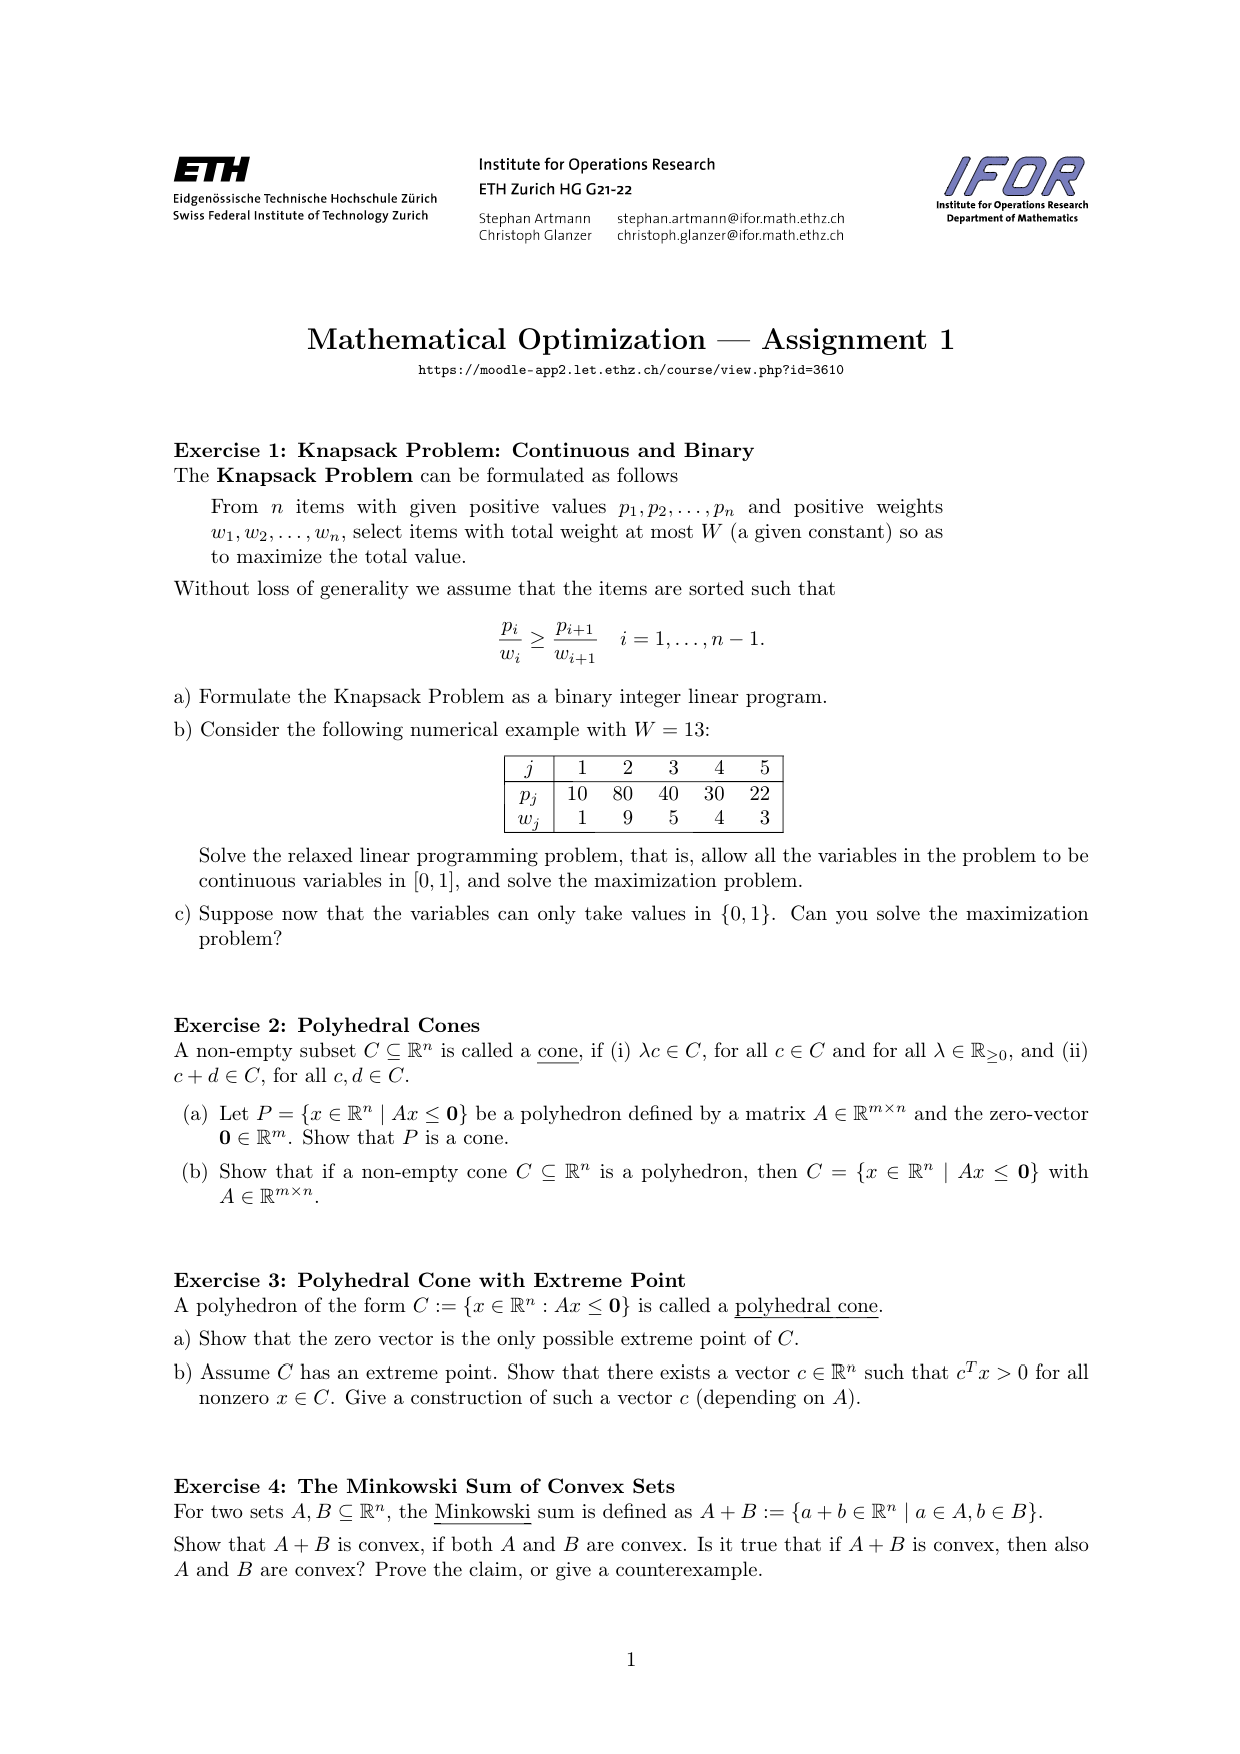
\includepdf[pages={1}]{docs/assignments/assignment1.pdf}

\subsection{Assignment 02 - 06/10/2017}
Topics: Projection of polyhedra, farka's lemma and standard form of polyhedra. 
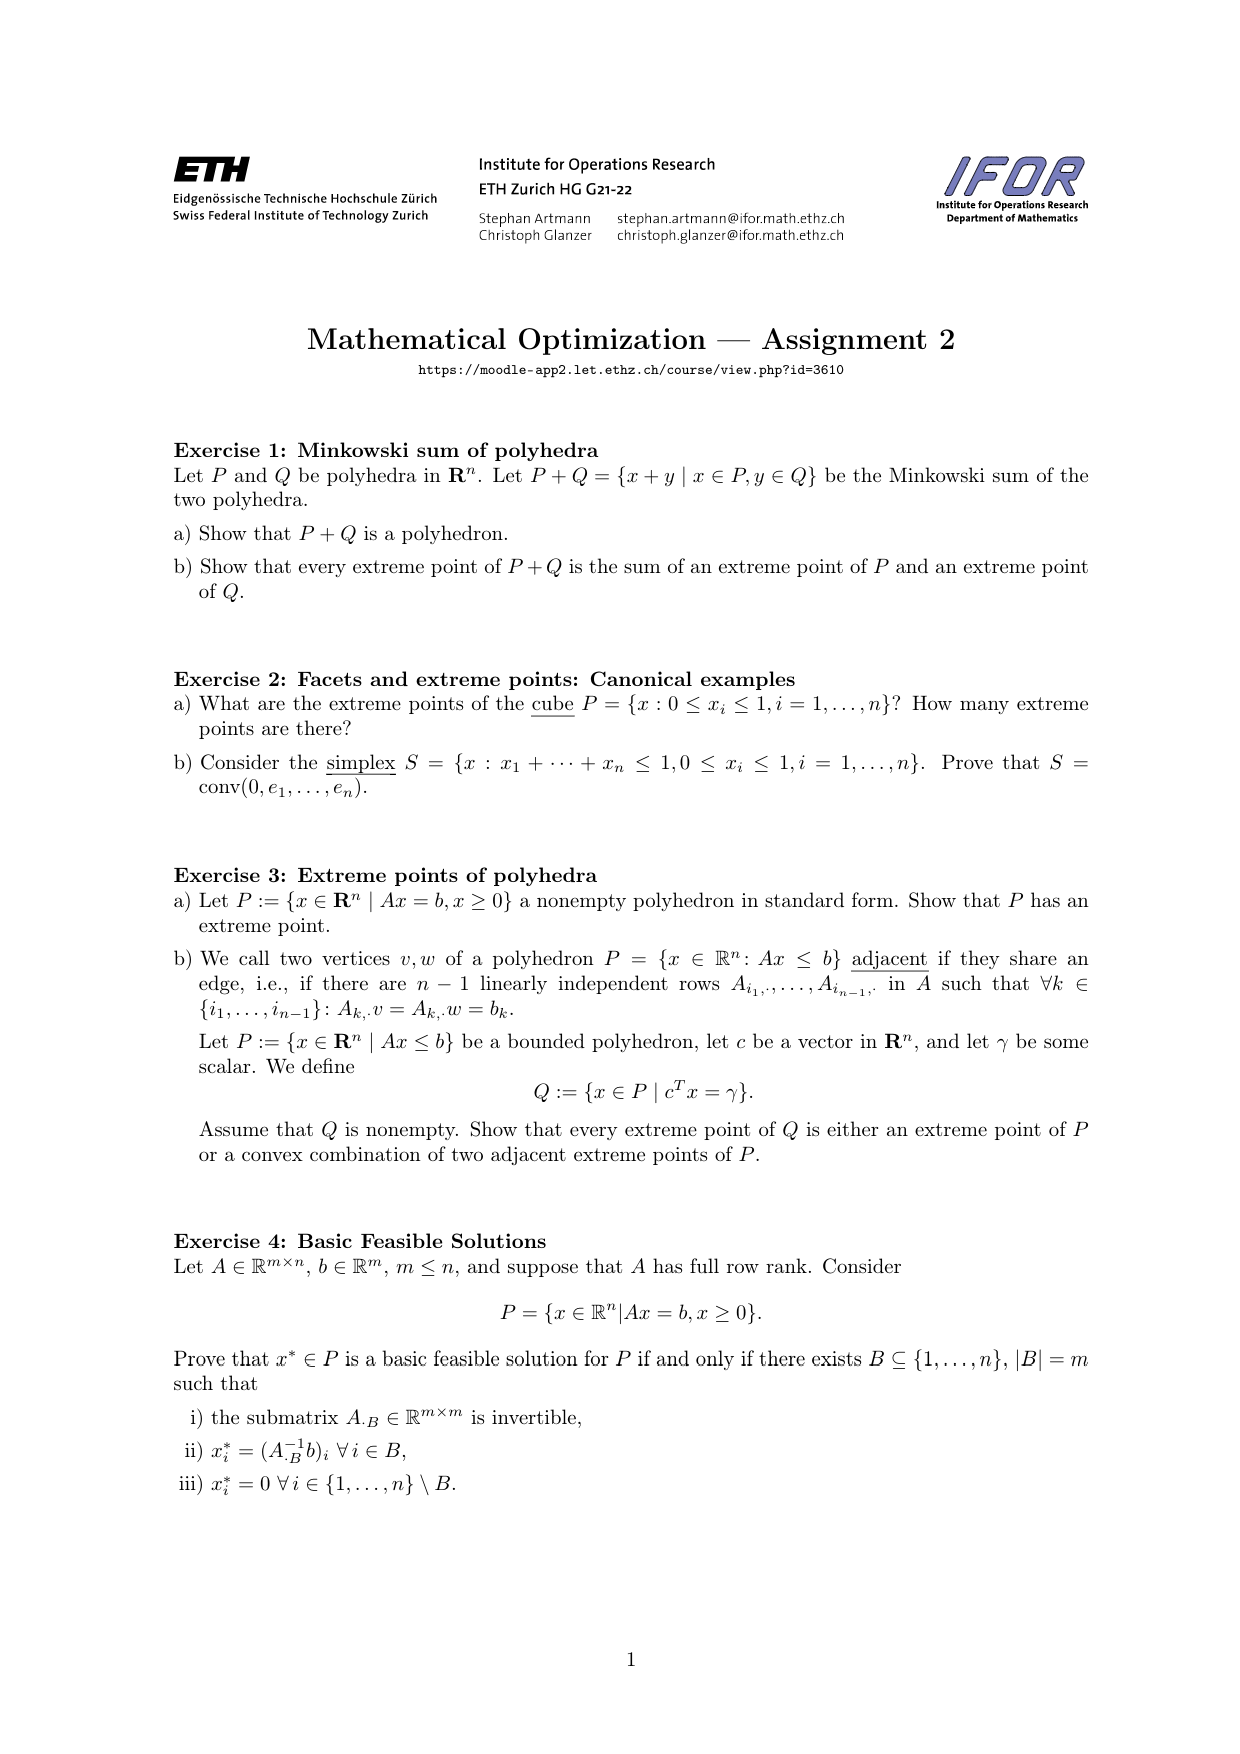
\includepdf[pages={1}]{docs/assignments/assignment2.pdf}

\subsection{Assignment 03 - 13/10/2017}
Topics: Duality theorem and representation of polyhedra
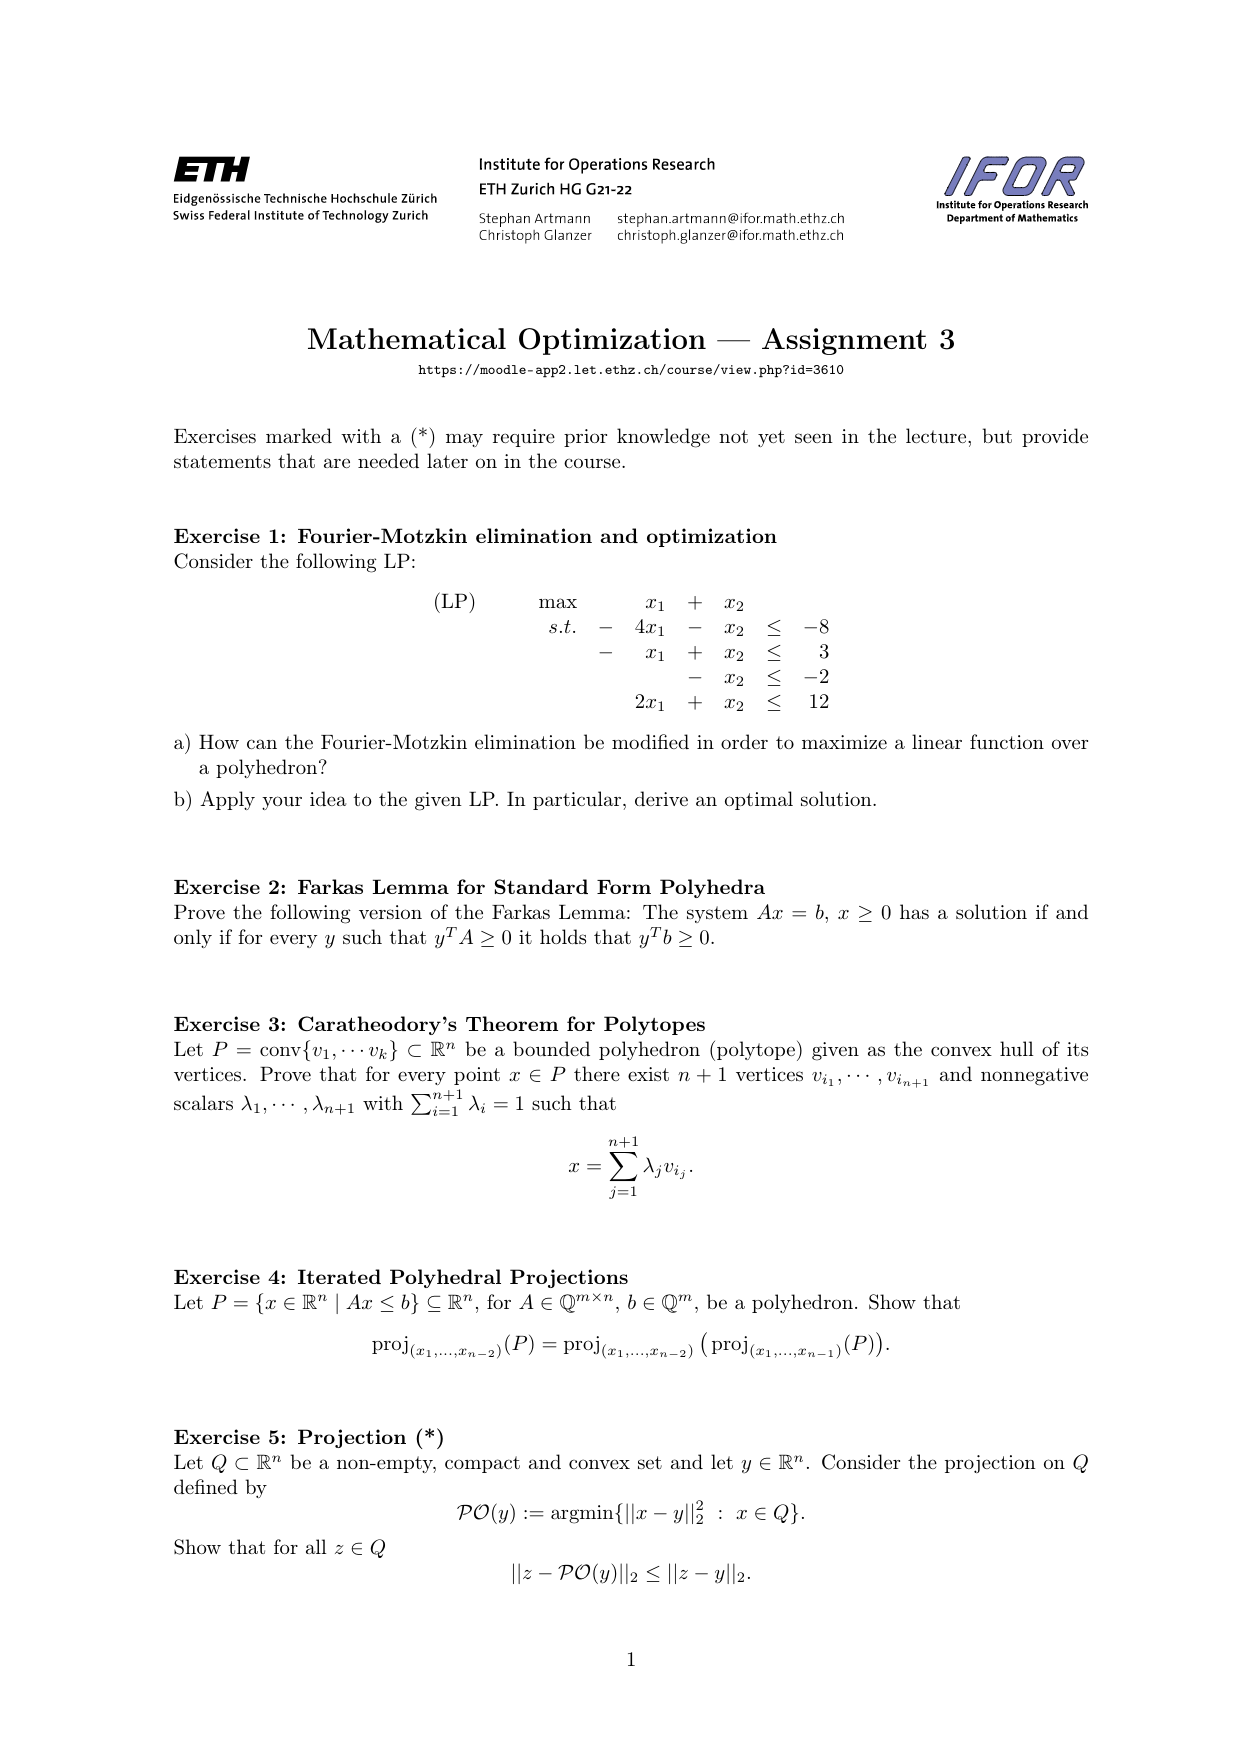
\includepdf[pages={1}]{docs/assignments/assignment3.pdf}

\subsection{Assignment 04 - 20/10/2017}
Topics: Simplex algorithm I and II.
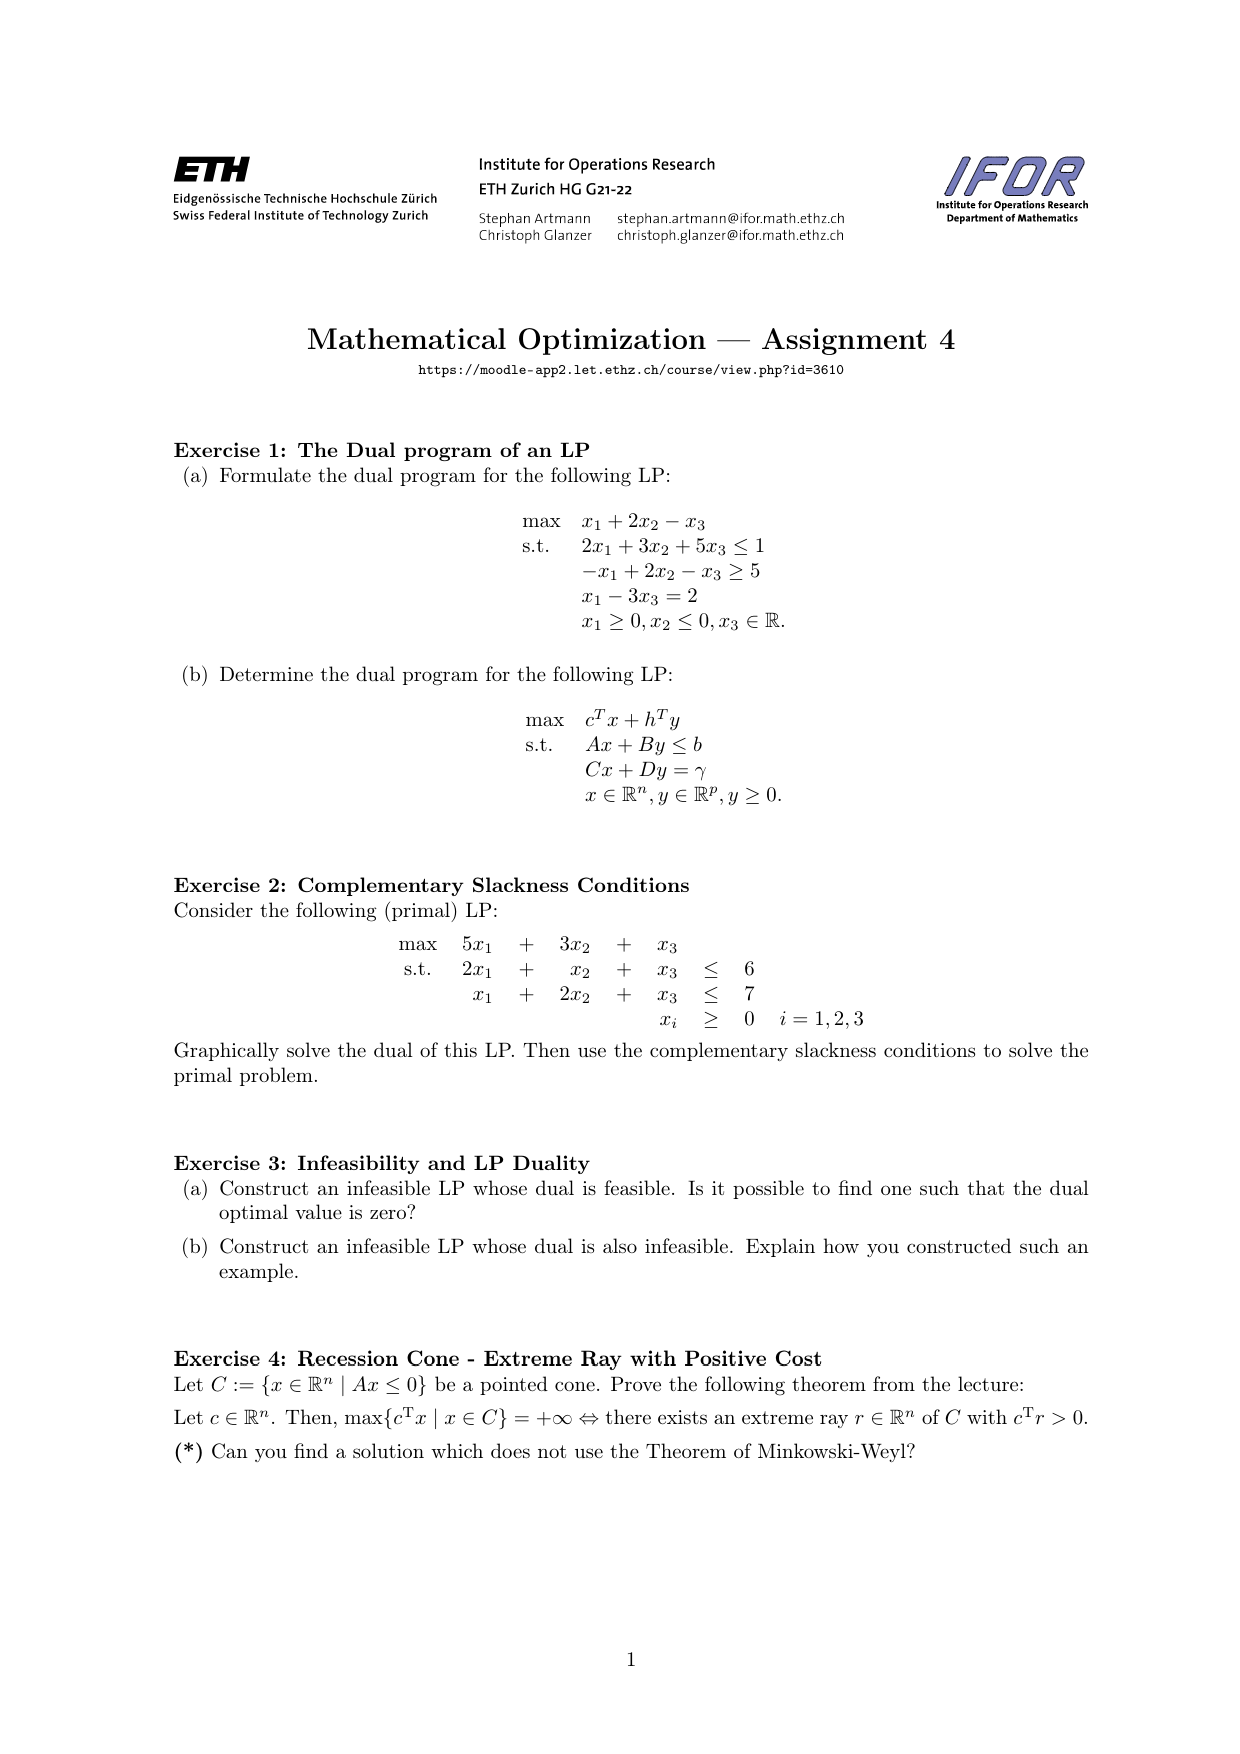
\includepdf[pages={1}]{docs/assignments/assignment4.pdf}

\subsection{Assignment 05 - 27/10/2017}
Topics: Simplex algorithm III and IV.
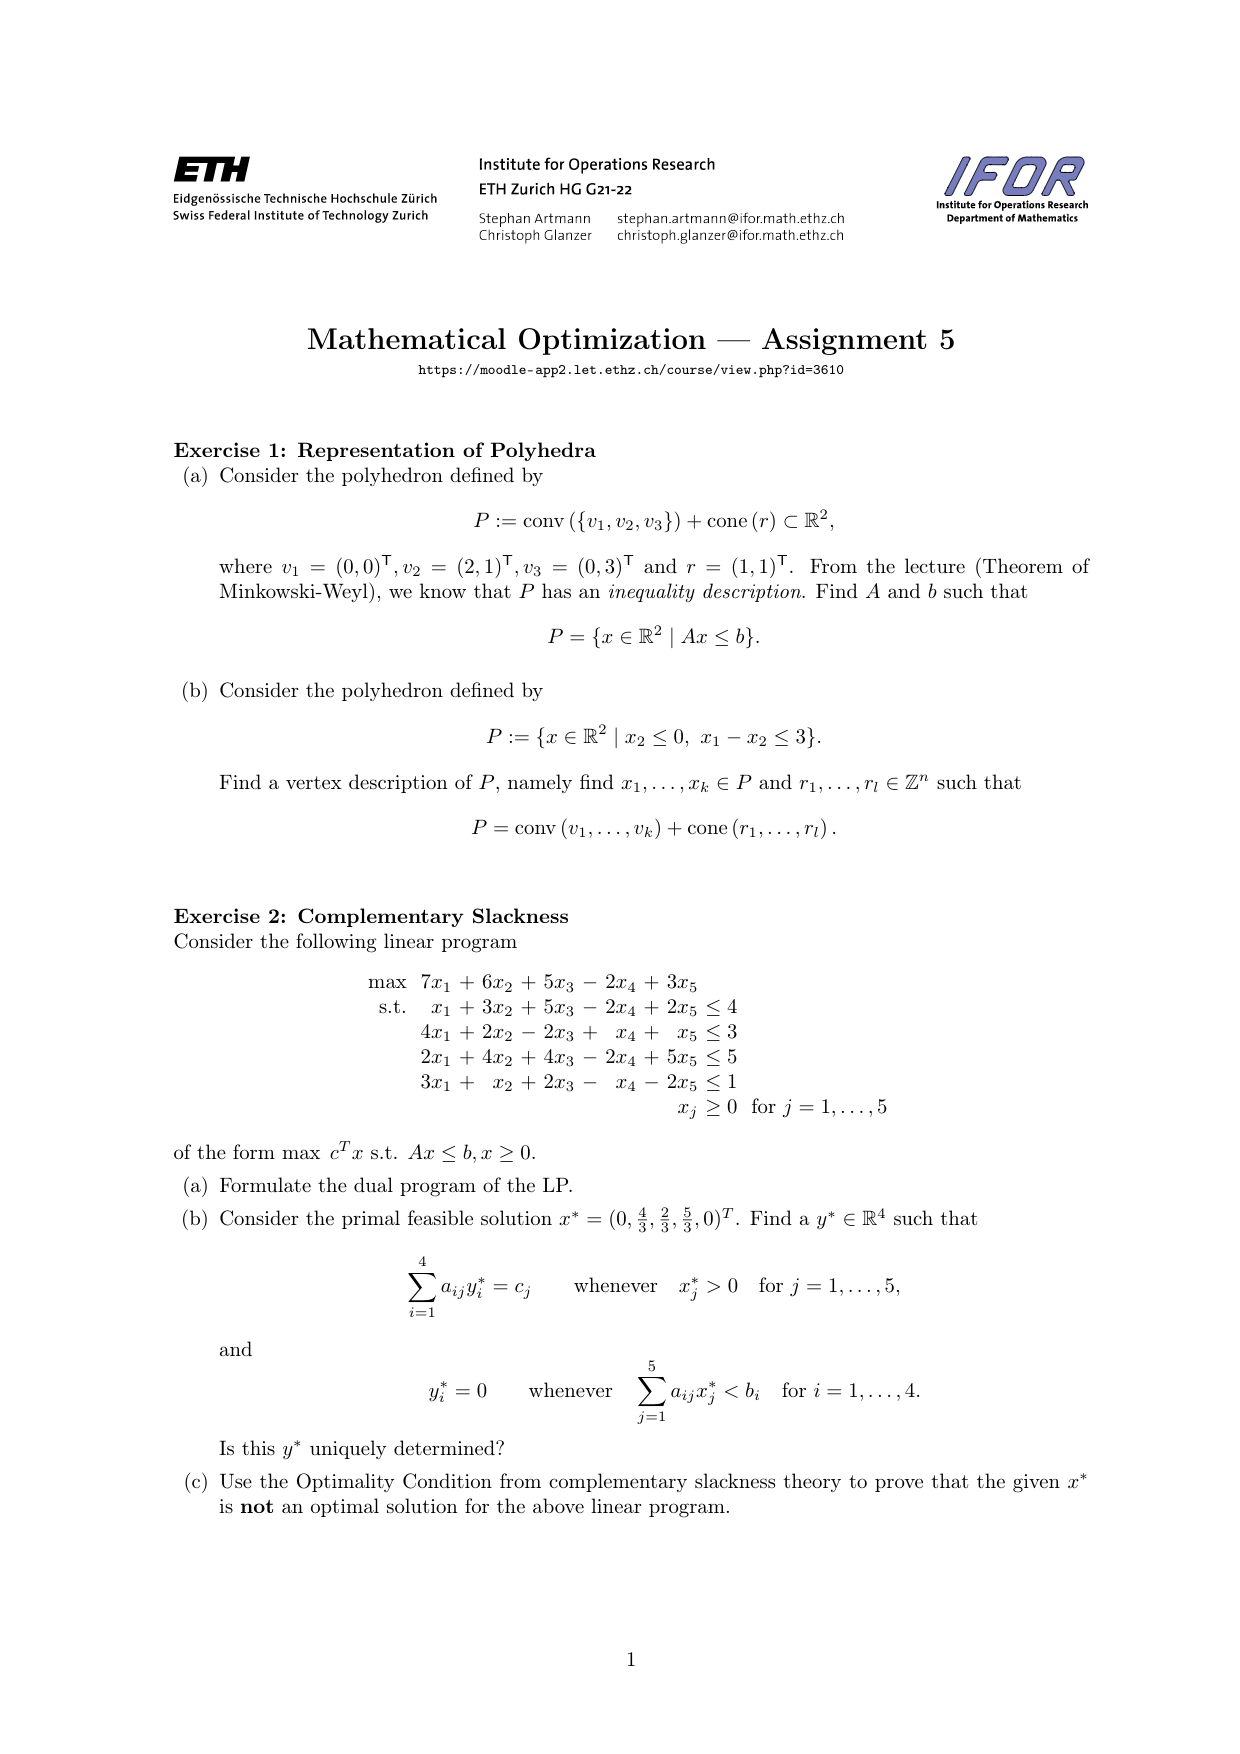
\includepdf[pages={1-2}]{docs/assignments/assignment5.pdf}

\subsection{Assignment 06 - 03/11/2017}
Topics: Interior point methods, convex optimization and the newton method.
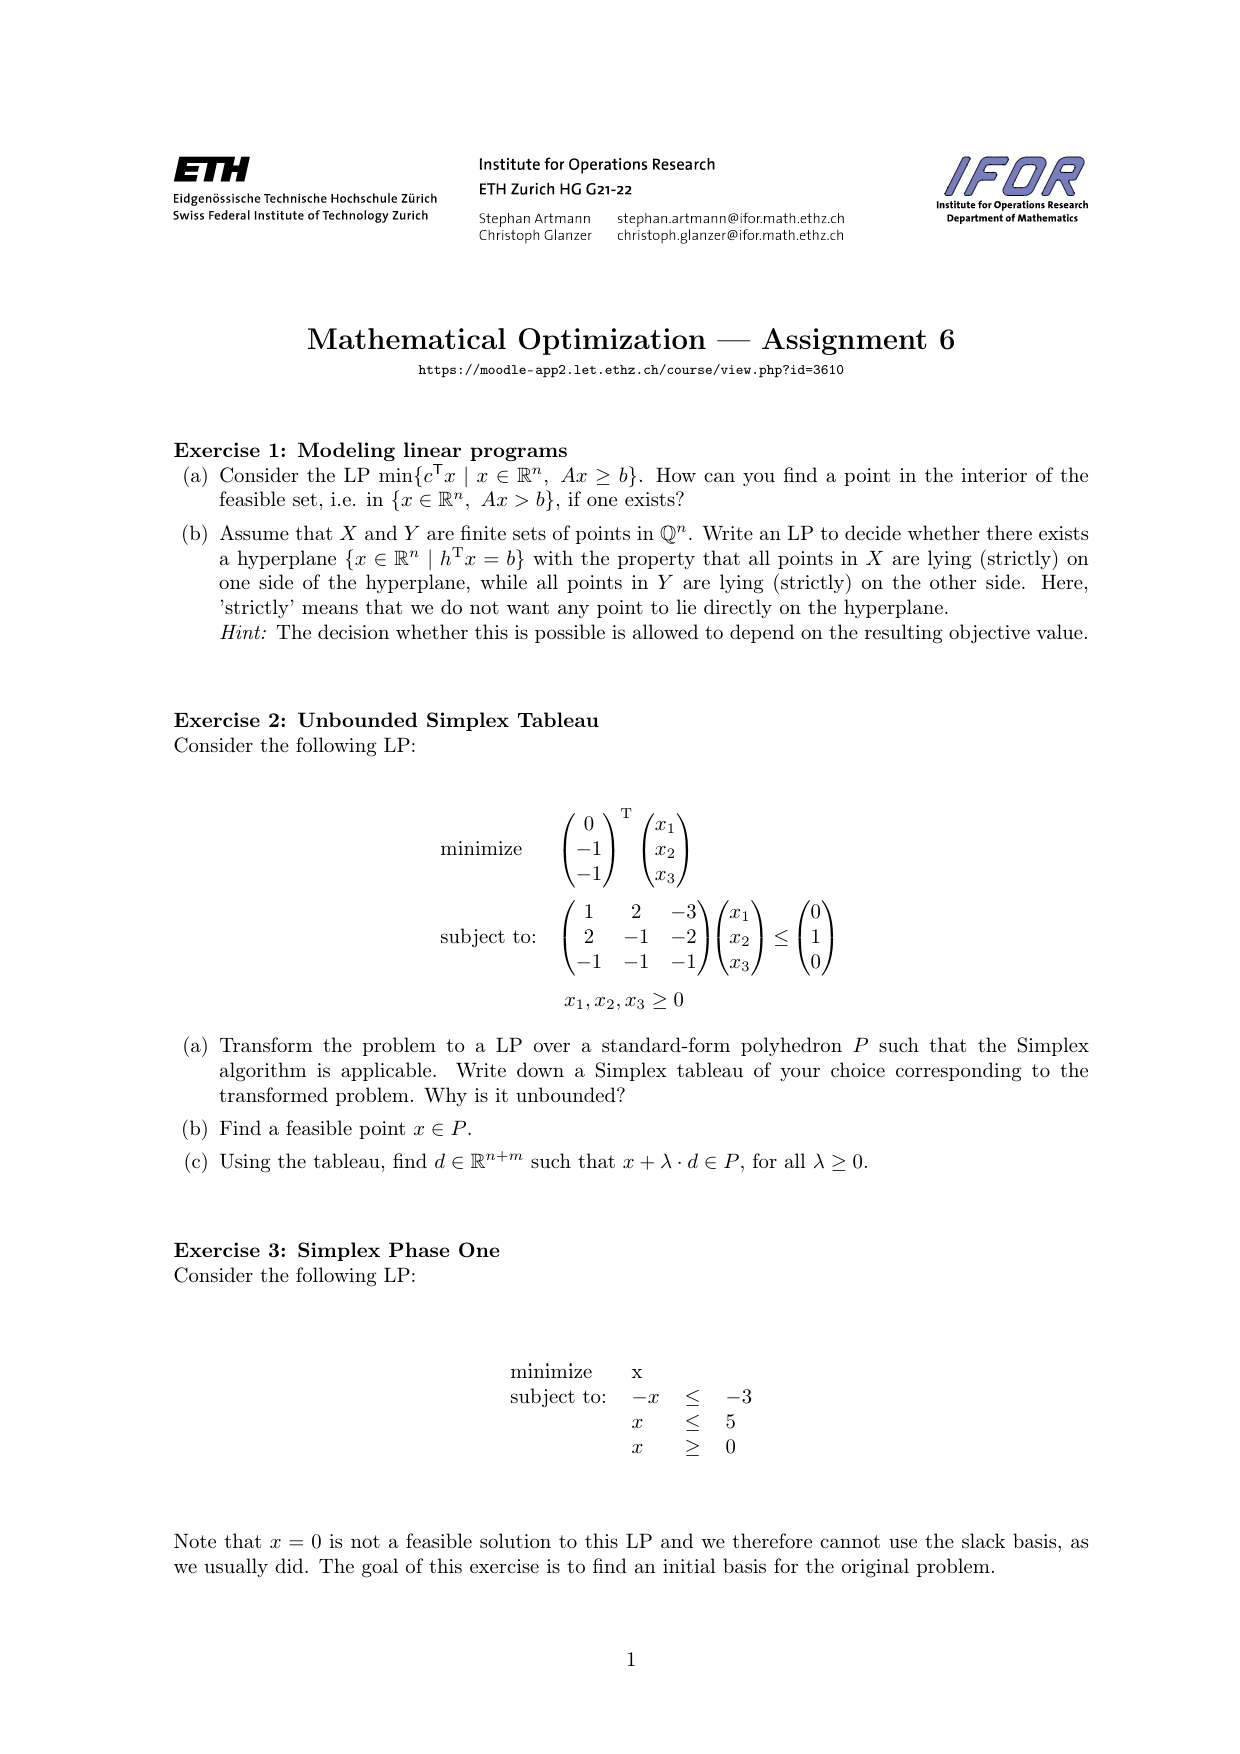
\includepdf[pages={1-2}]{docs/assignments/assignment6.pdf}

\subsection{Assignment 07 - 10/11/2017}
Topics: Convex optimization duality I and II.
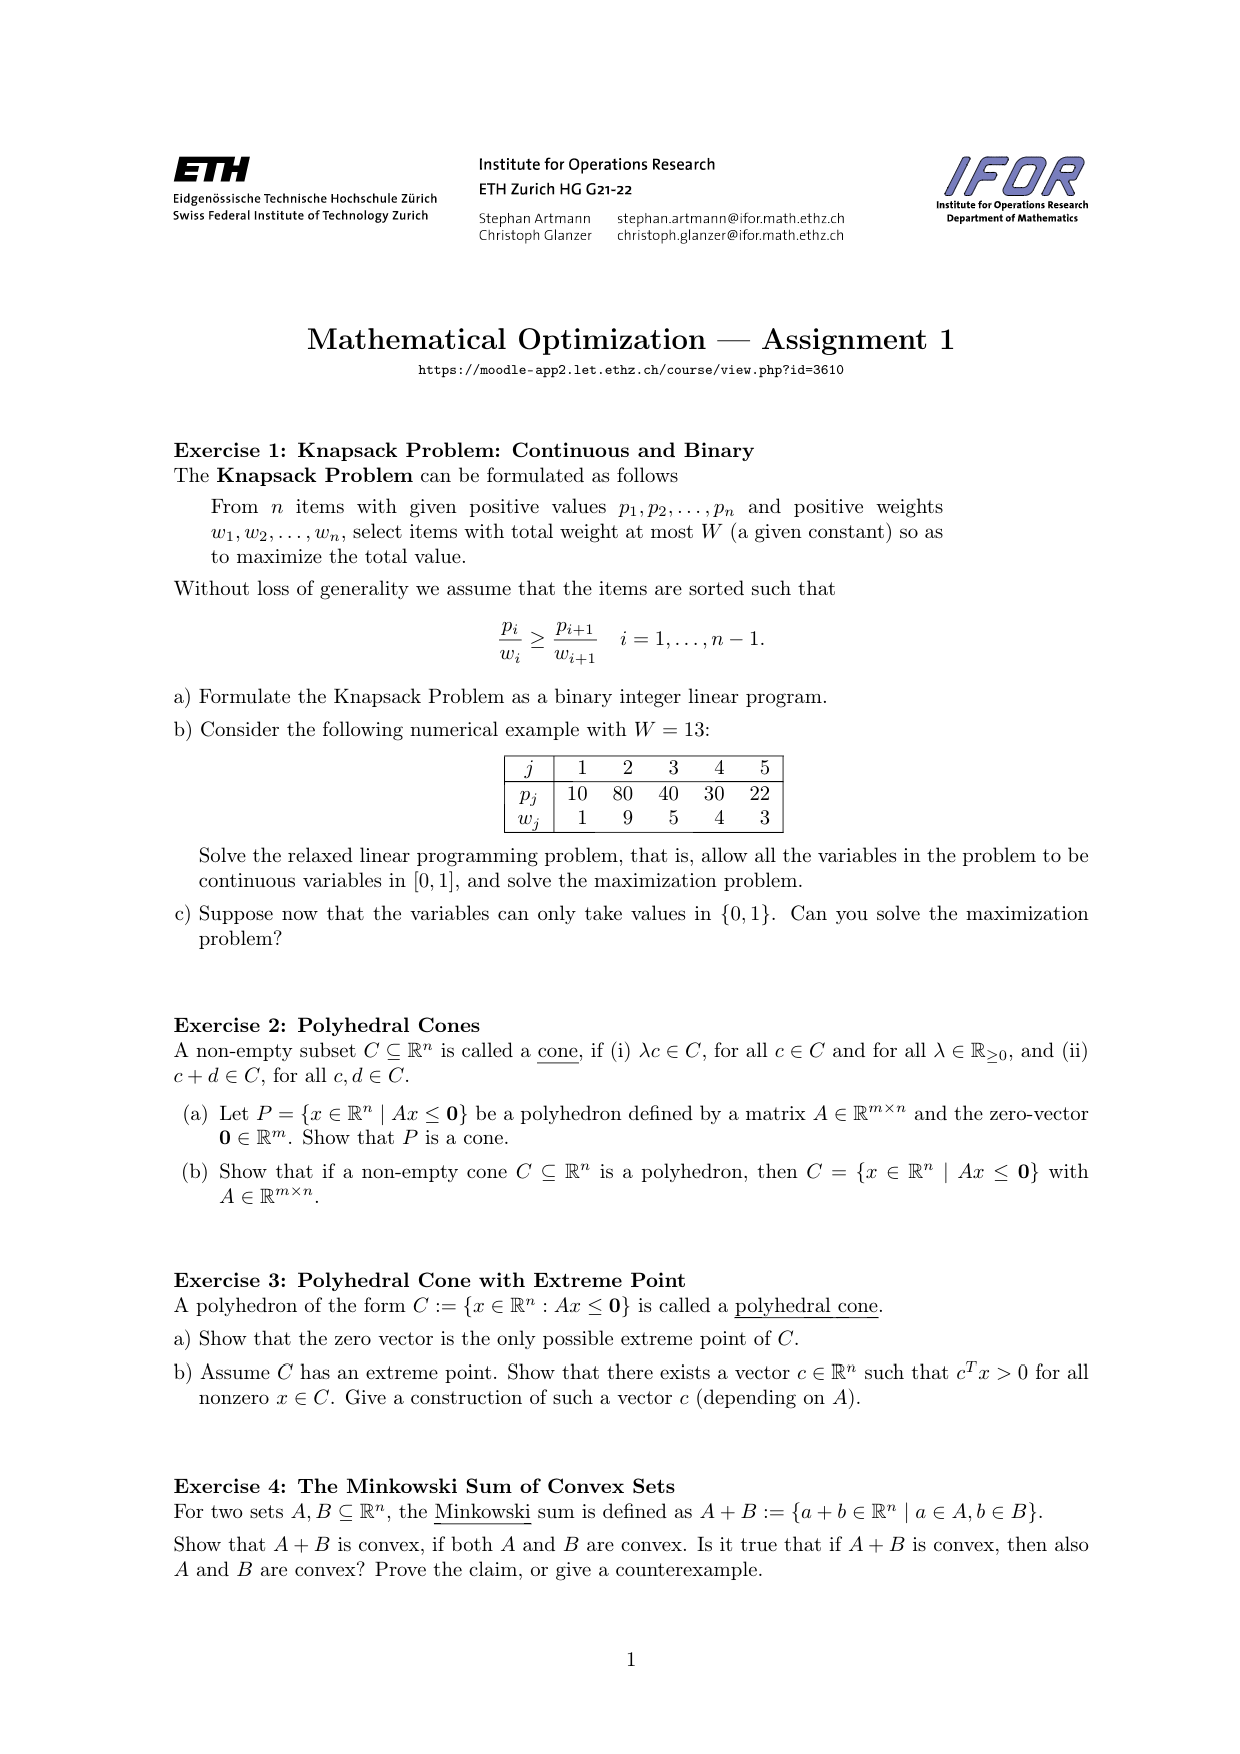
\includepdf[pages={1}]{docs/assignments/assignment1.pdf}

\subsection{Assignment 08 - 17/11/2017}
Topics: Total unimodular matrices and applications.
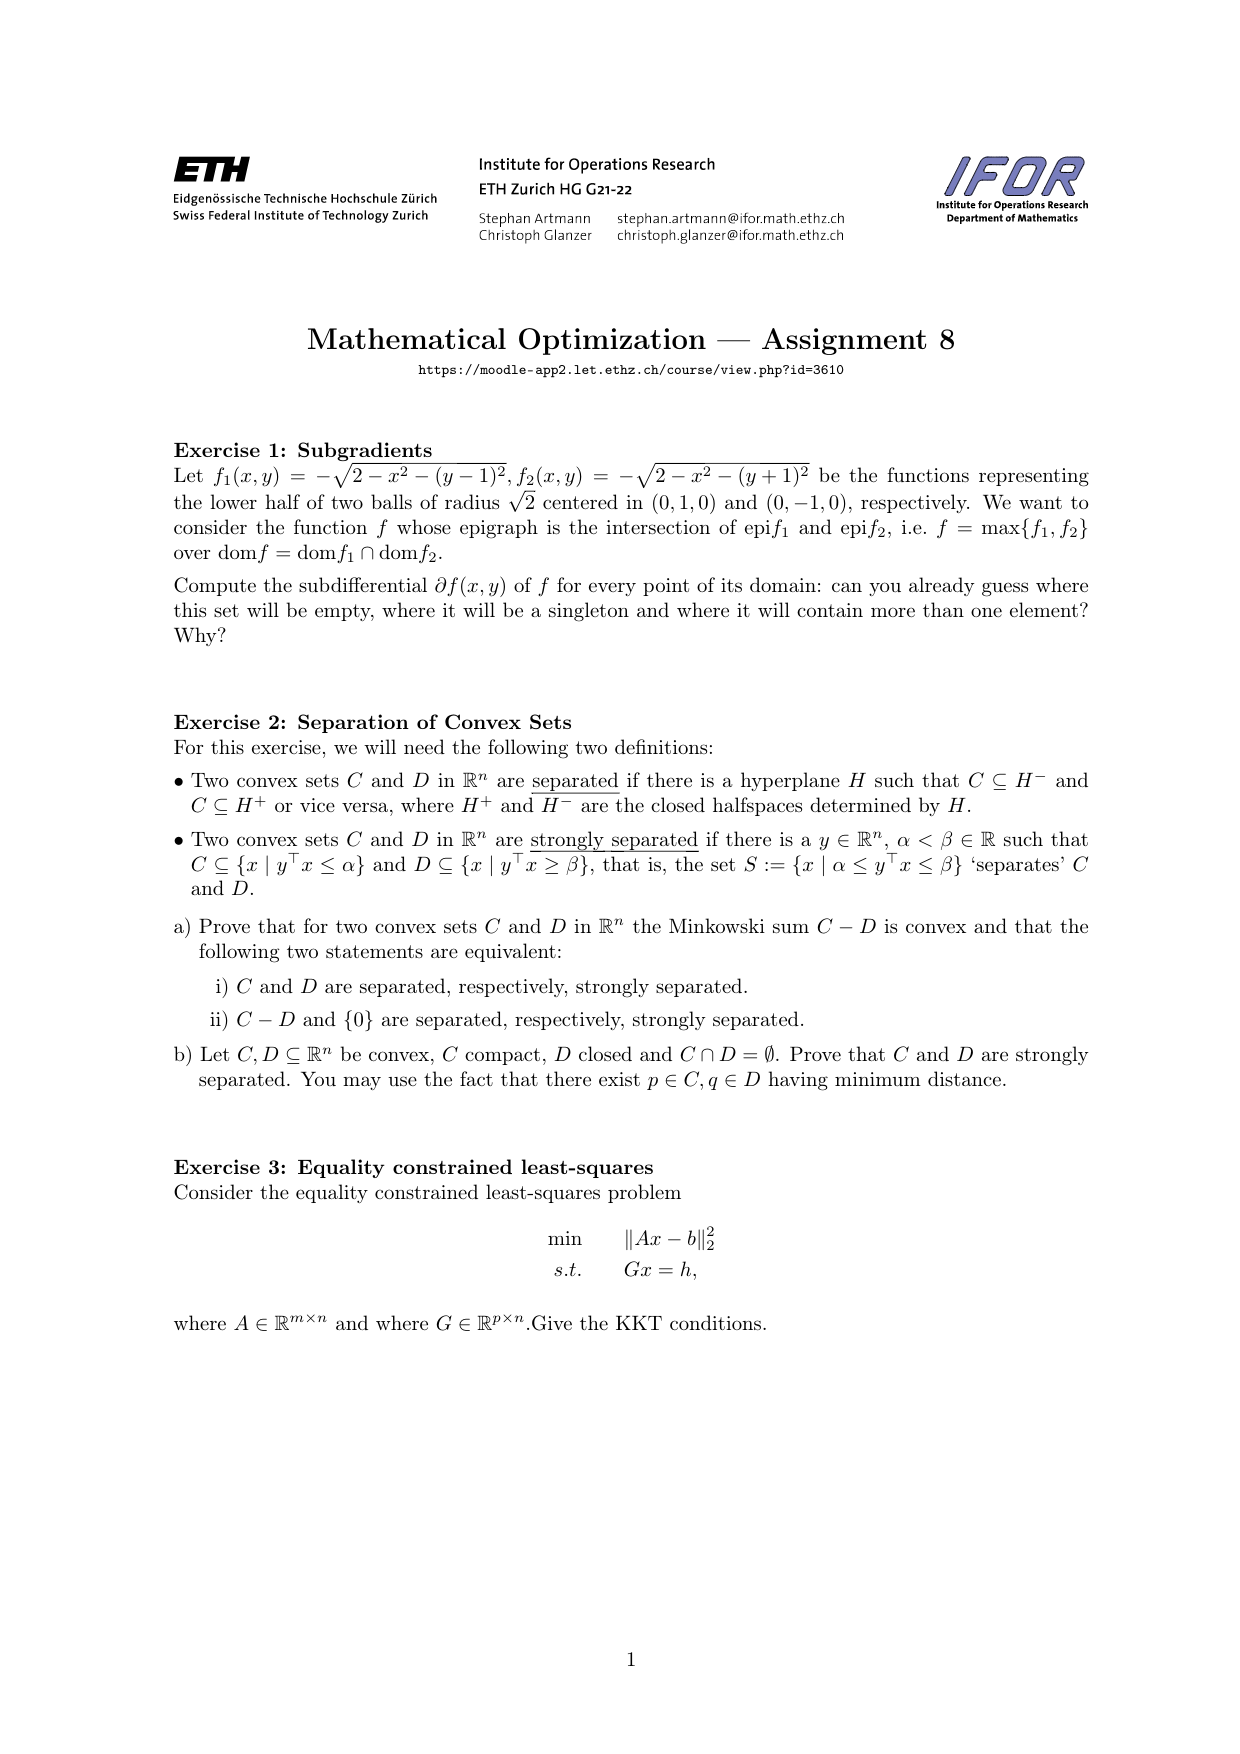
\includepdf[pages={1}]{docs/assignments/assignment8.pdf}

\subsection{Assignment 09 - 24/11/2017}
Topics: Algorithms for hard problems and polyhedral representation of discrete
optimization problems.
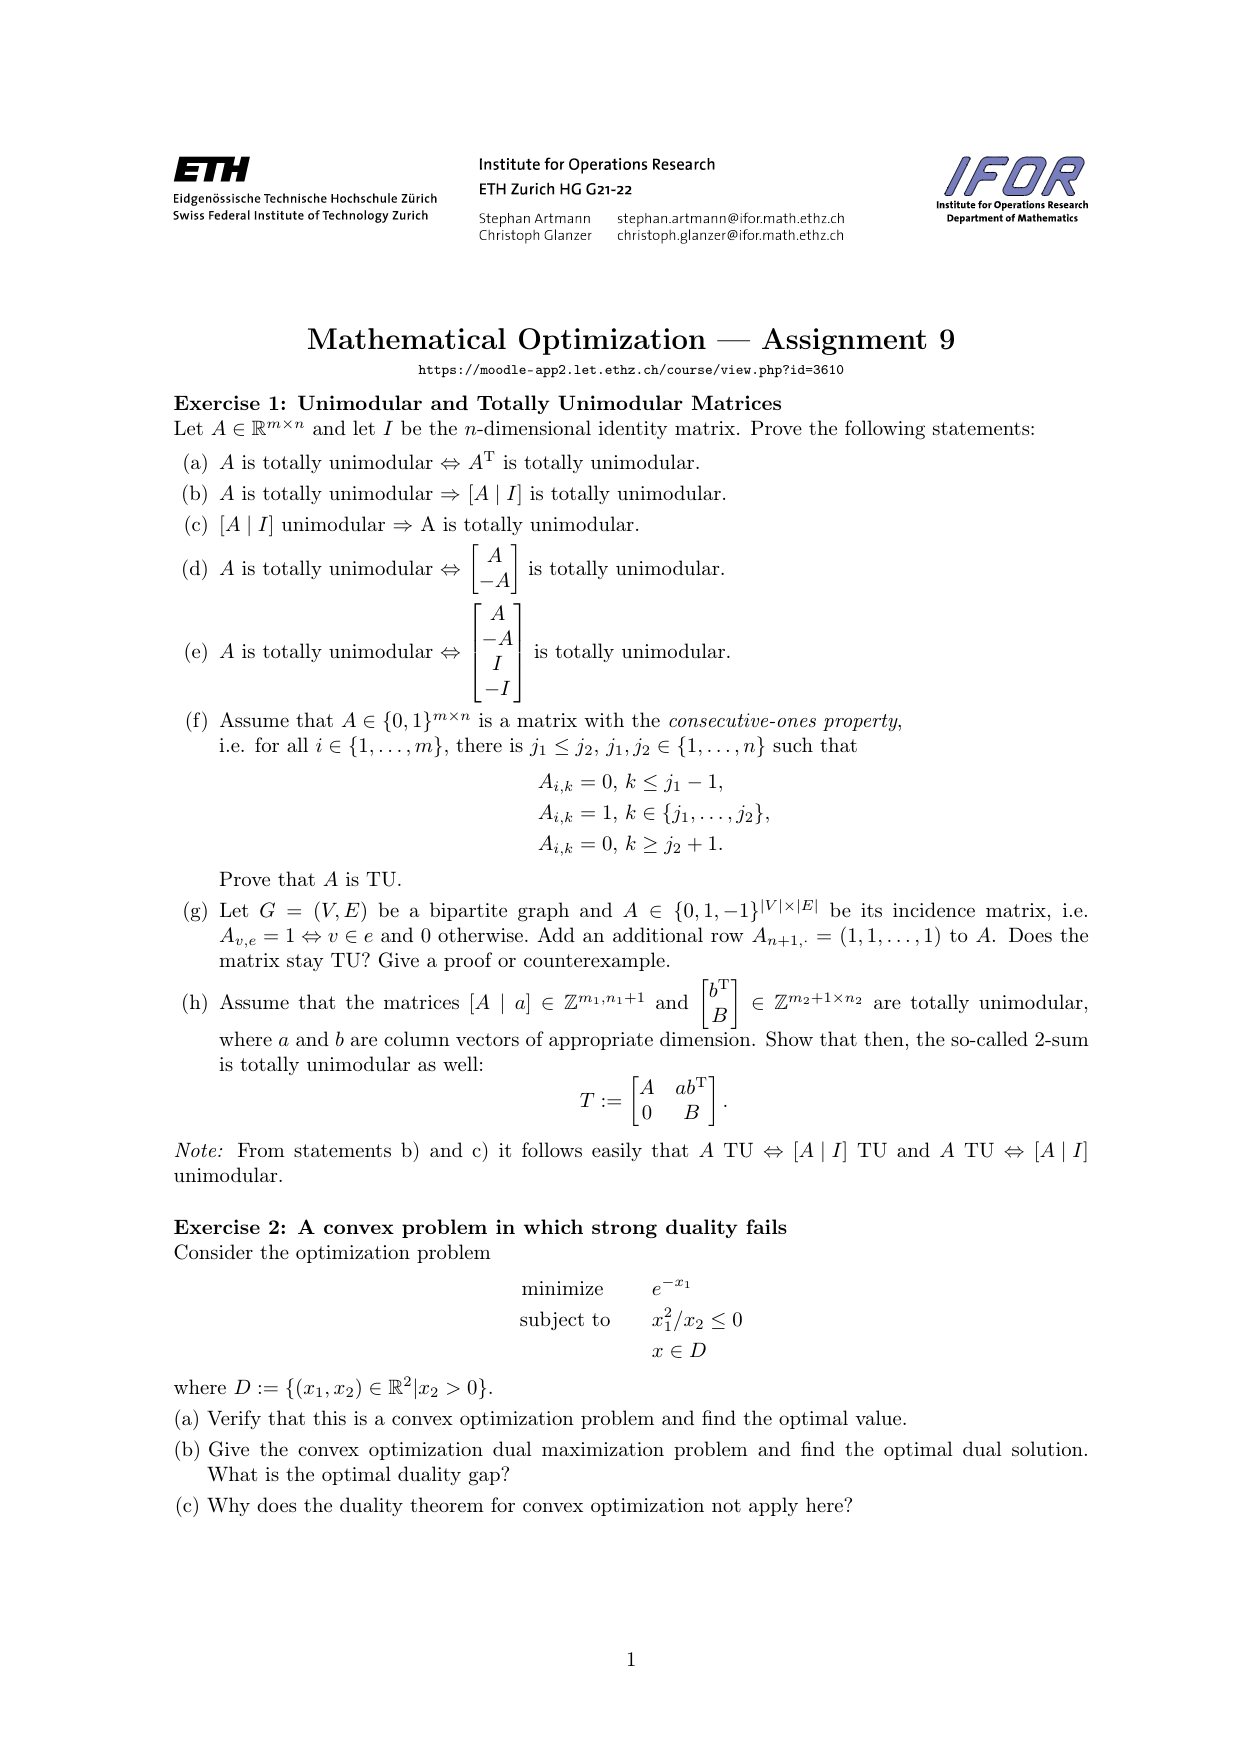
\includepdf[pages={1}]{docs/assignments/assignment9.pdf}

\subsection{Assignment 10 - 1/12/2017}
Topics: From linear to integer optimization and principles of cutting planes
generation.
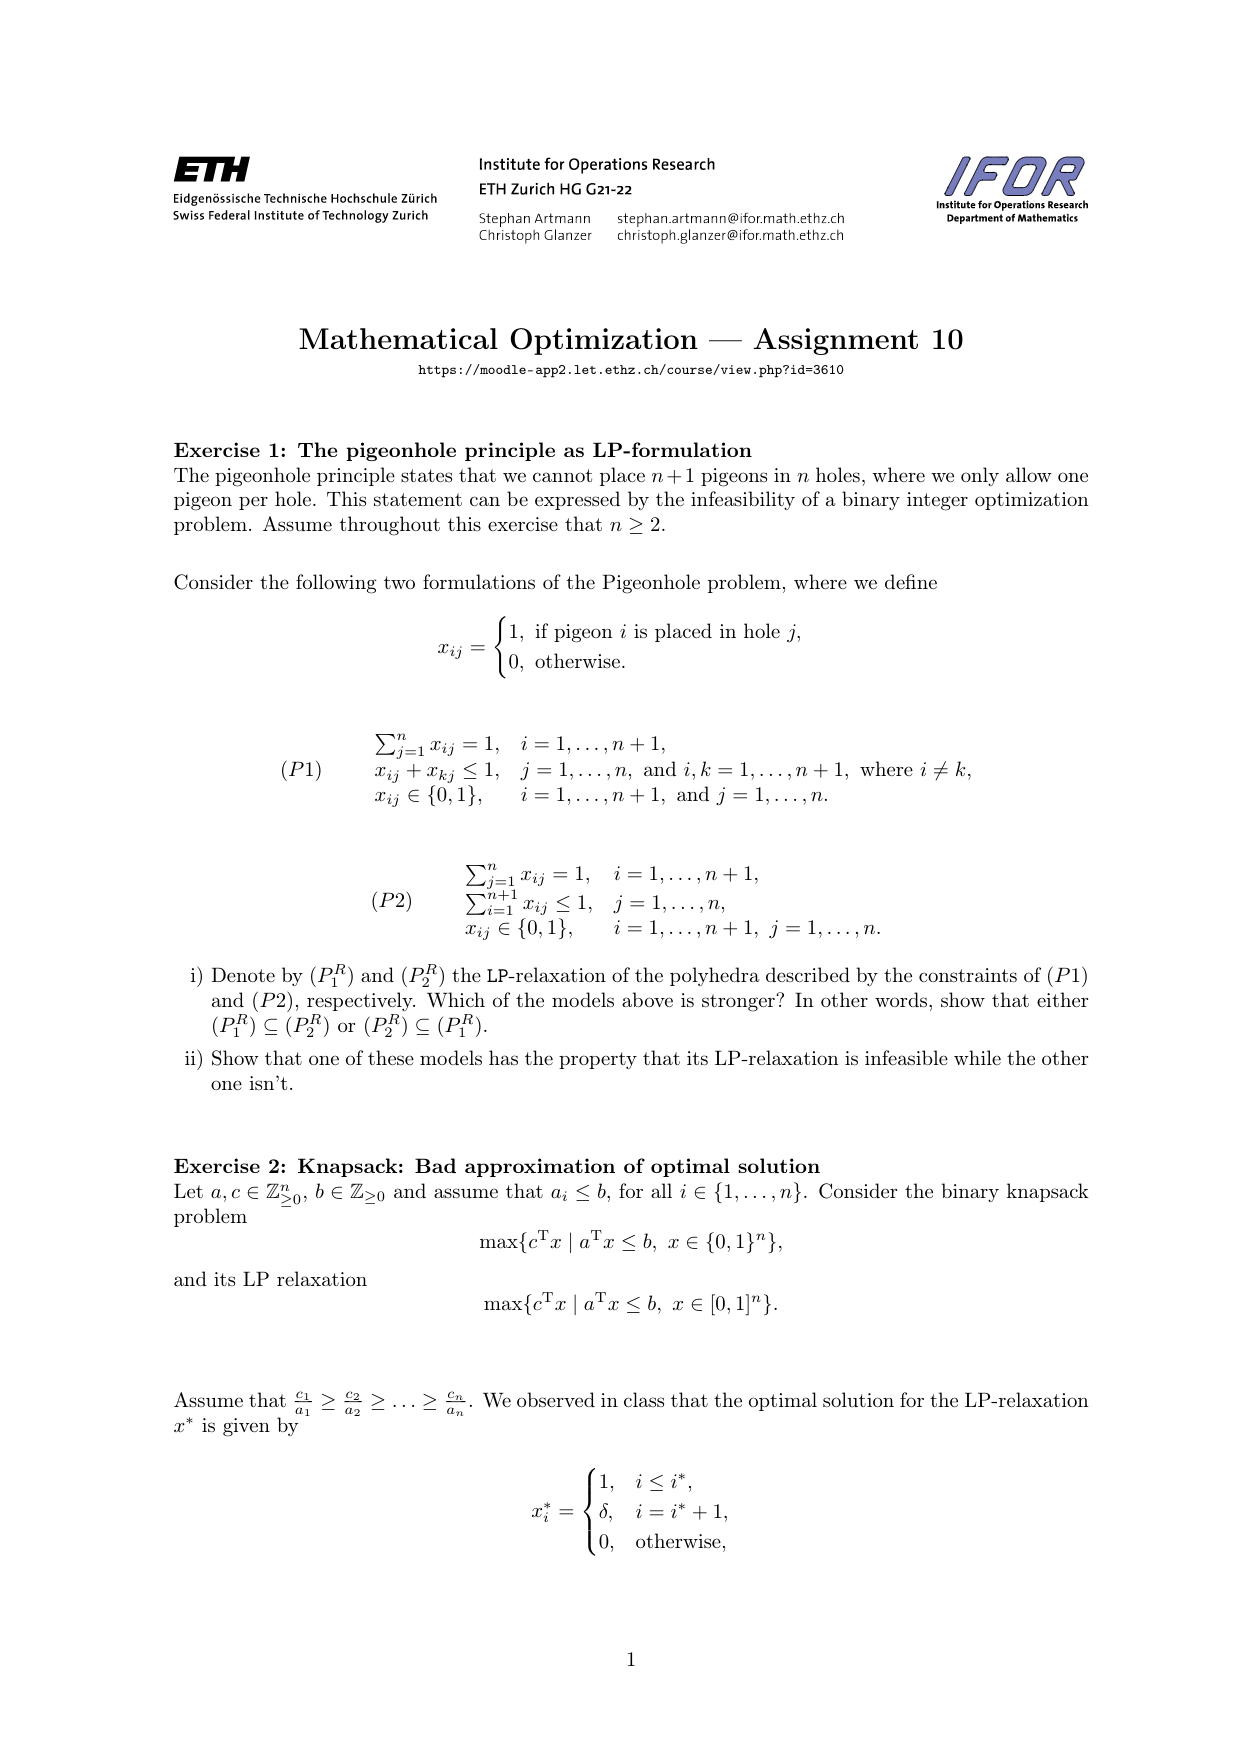
\includepdf[pages={1-2}]{docs/assignments/assignment10.pdf}

\subsection{Assignment 11 - 8/12/2017}
Topics: The lift and project method and independence systems and matroids.
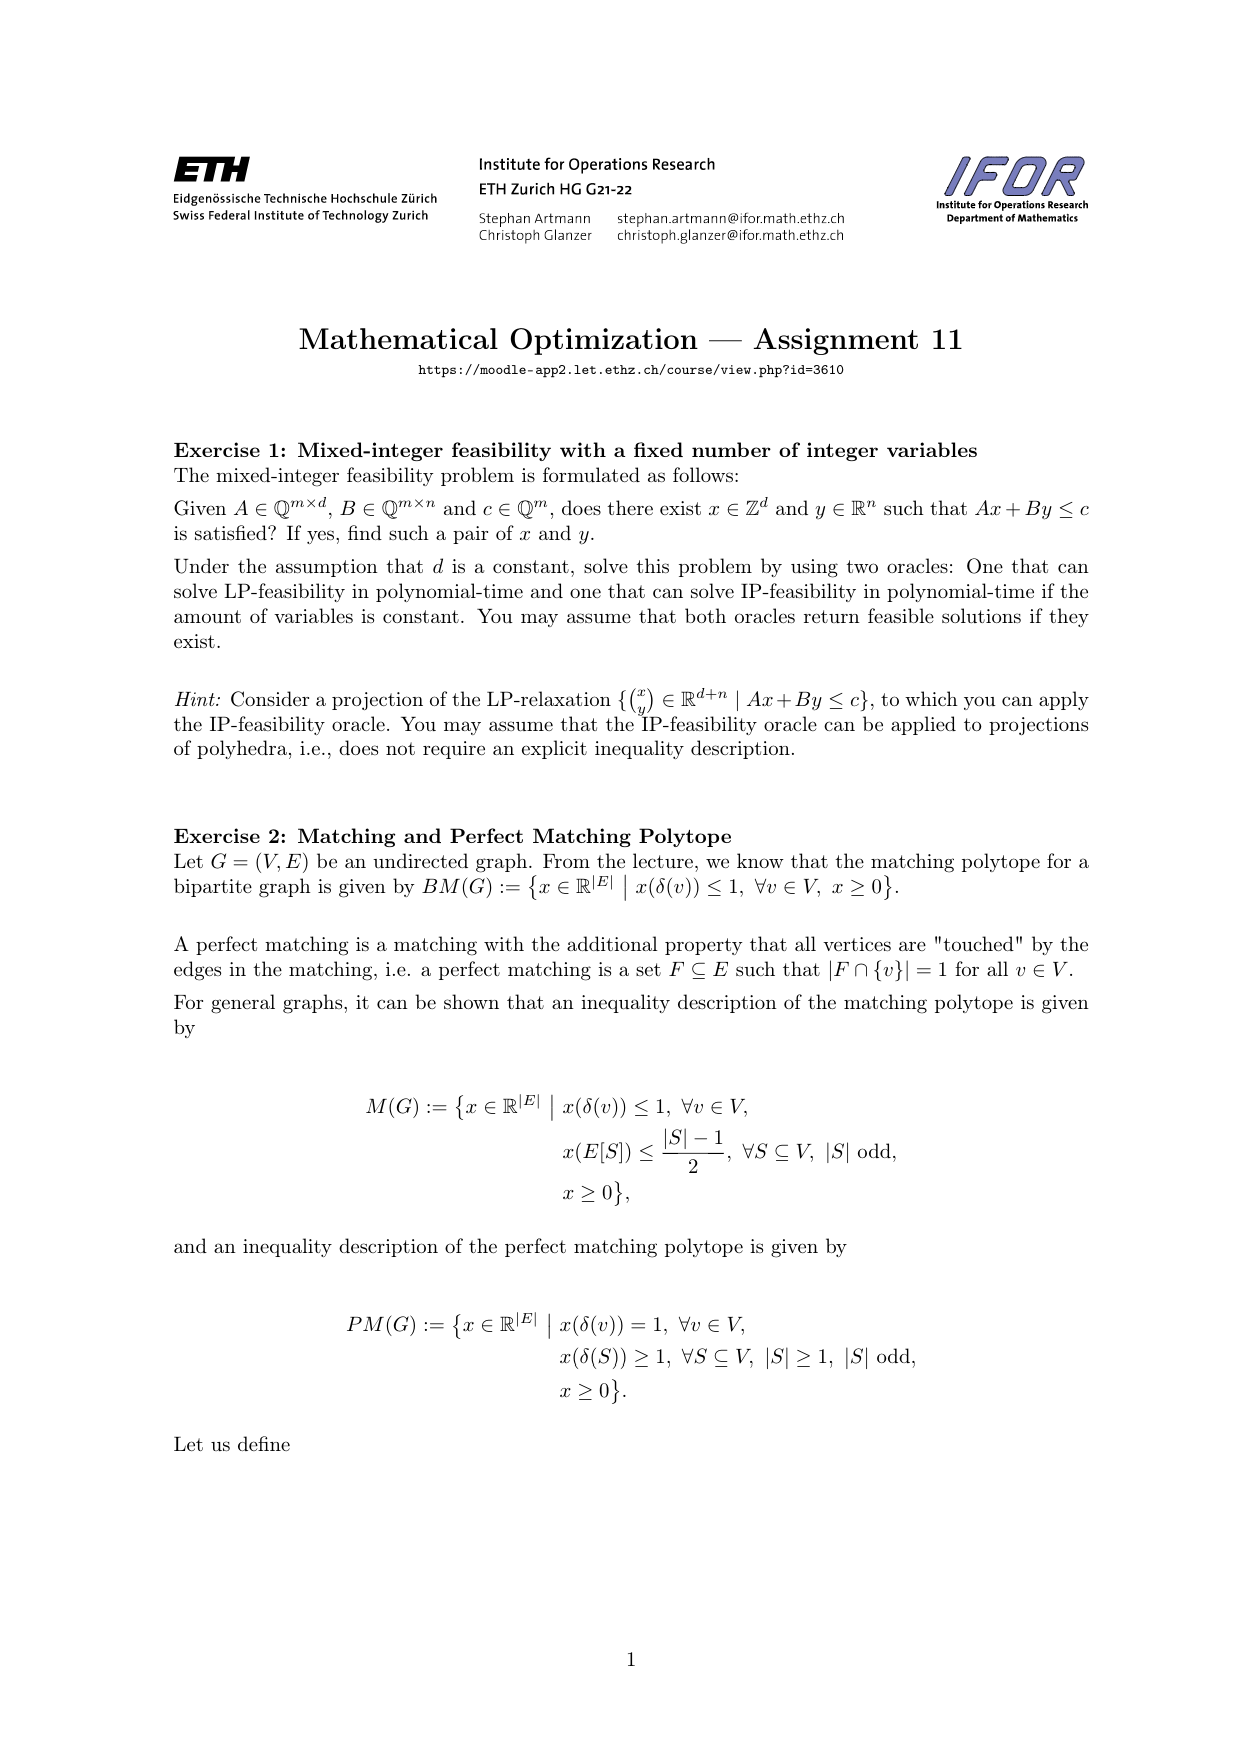
\includepdf[pages={1-2}]{docs/assignments/assignment11.pdf}

\subsection{Assignment 12 - 15/12/2017}
Topics: The intersection of two matroids and matching in (bipartite) graphs.
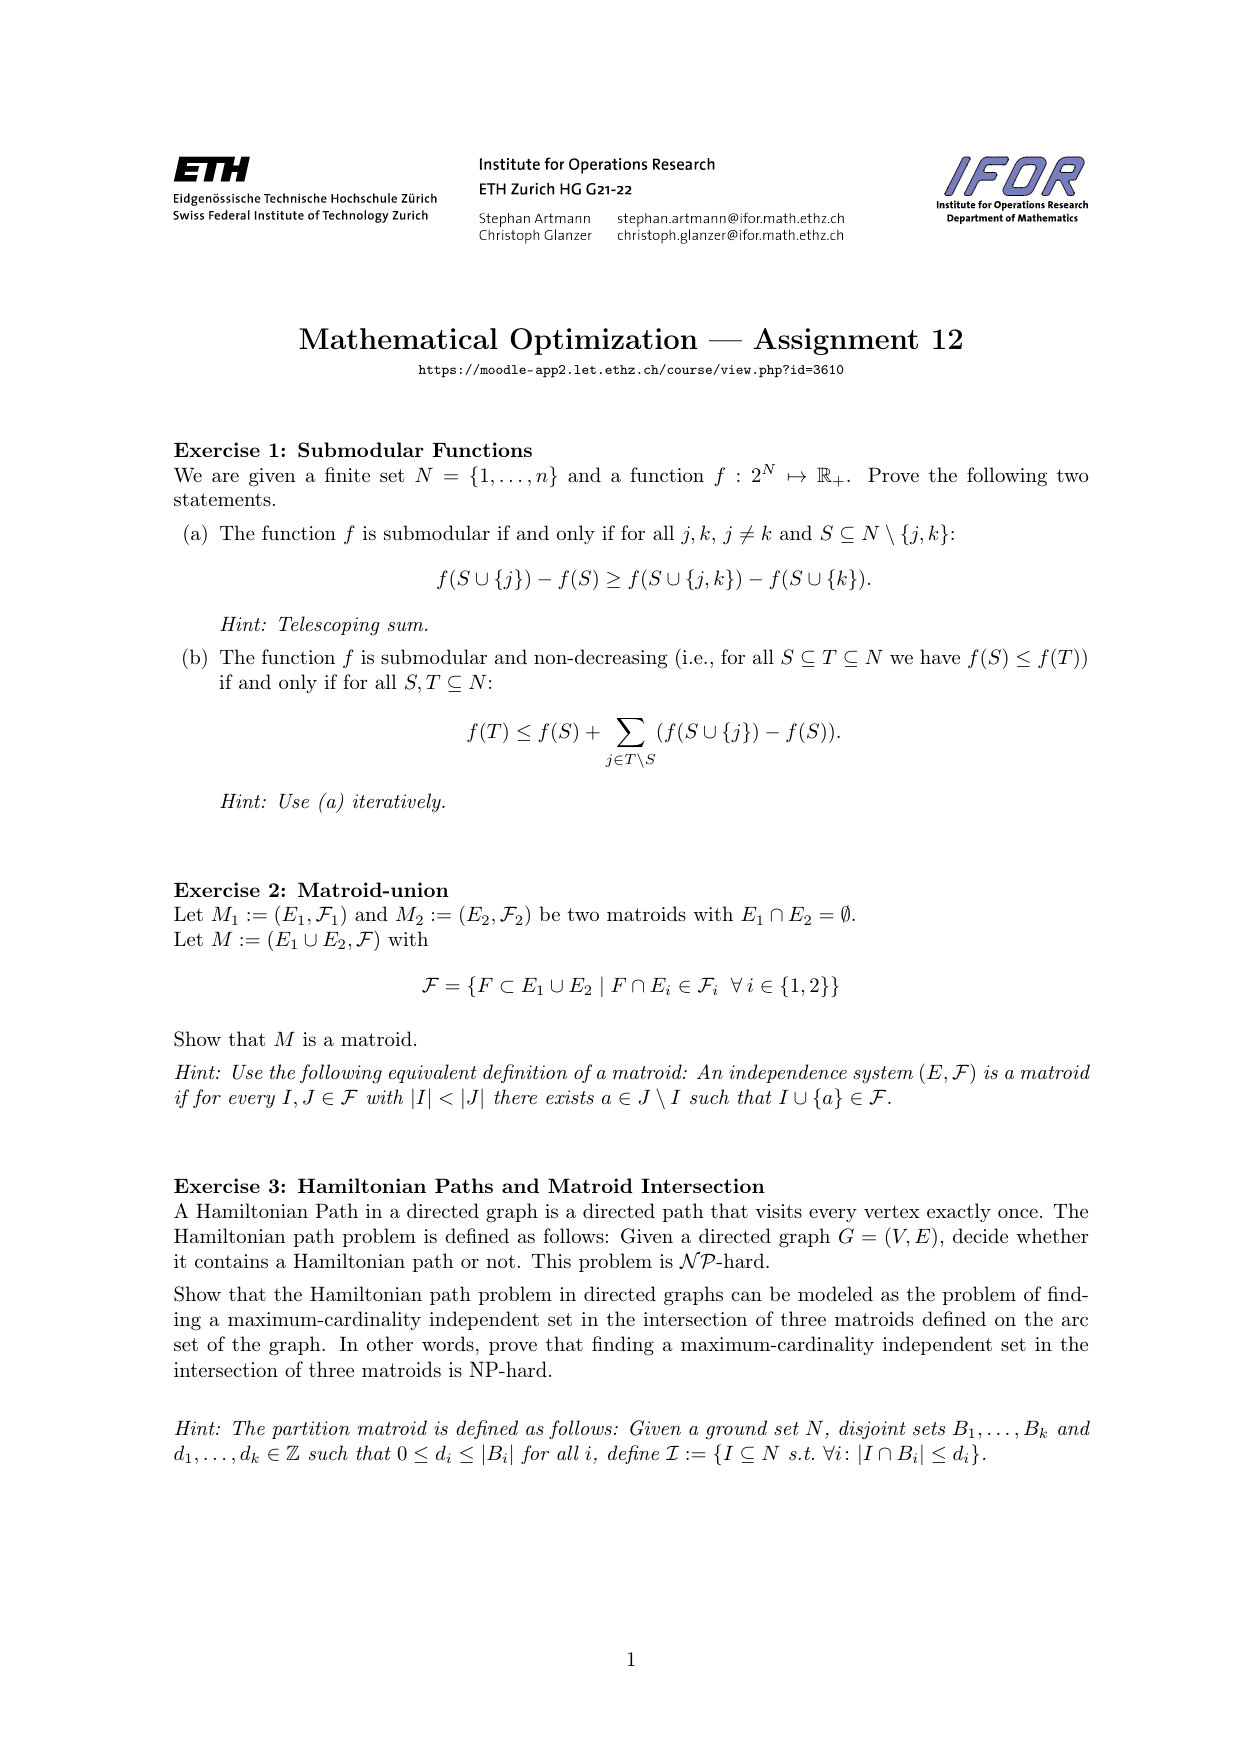
\includepdf[pages={1}]{docs/assignments/assignment12.pdf}

\section{Solutions}
% past exercises and sample solutions
\subsection{Assignment 01}
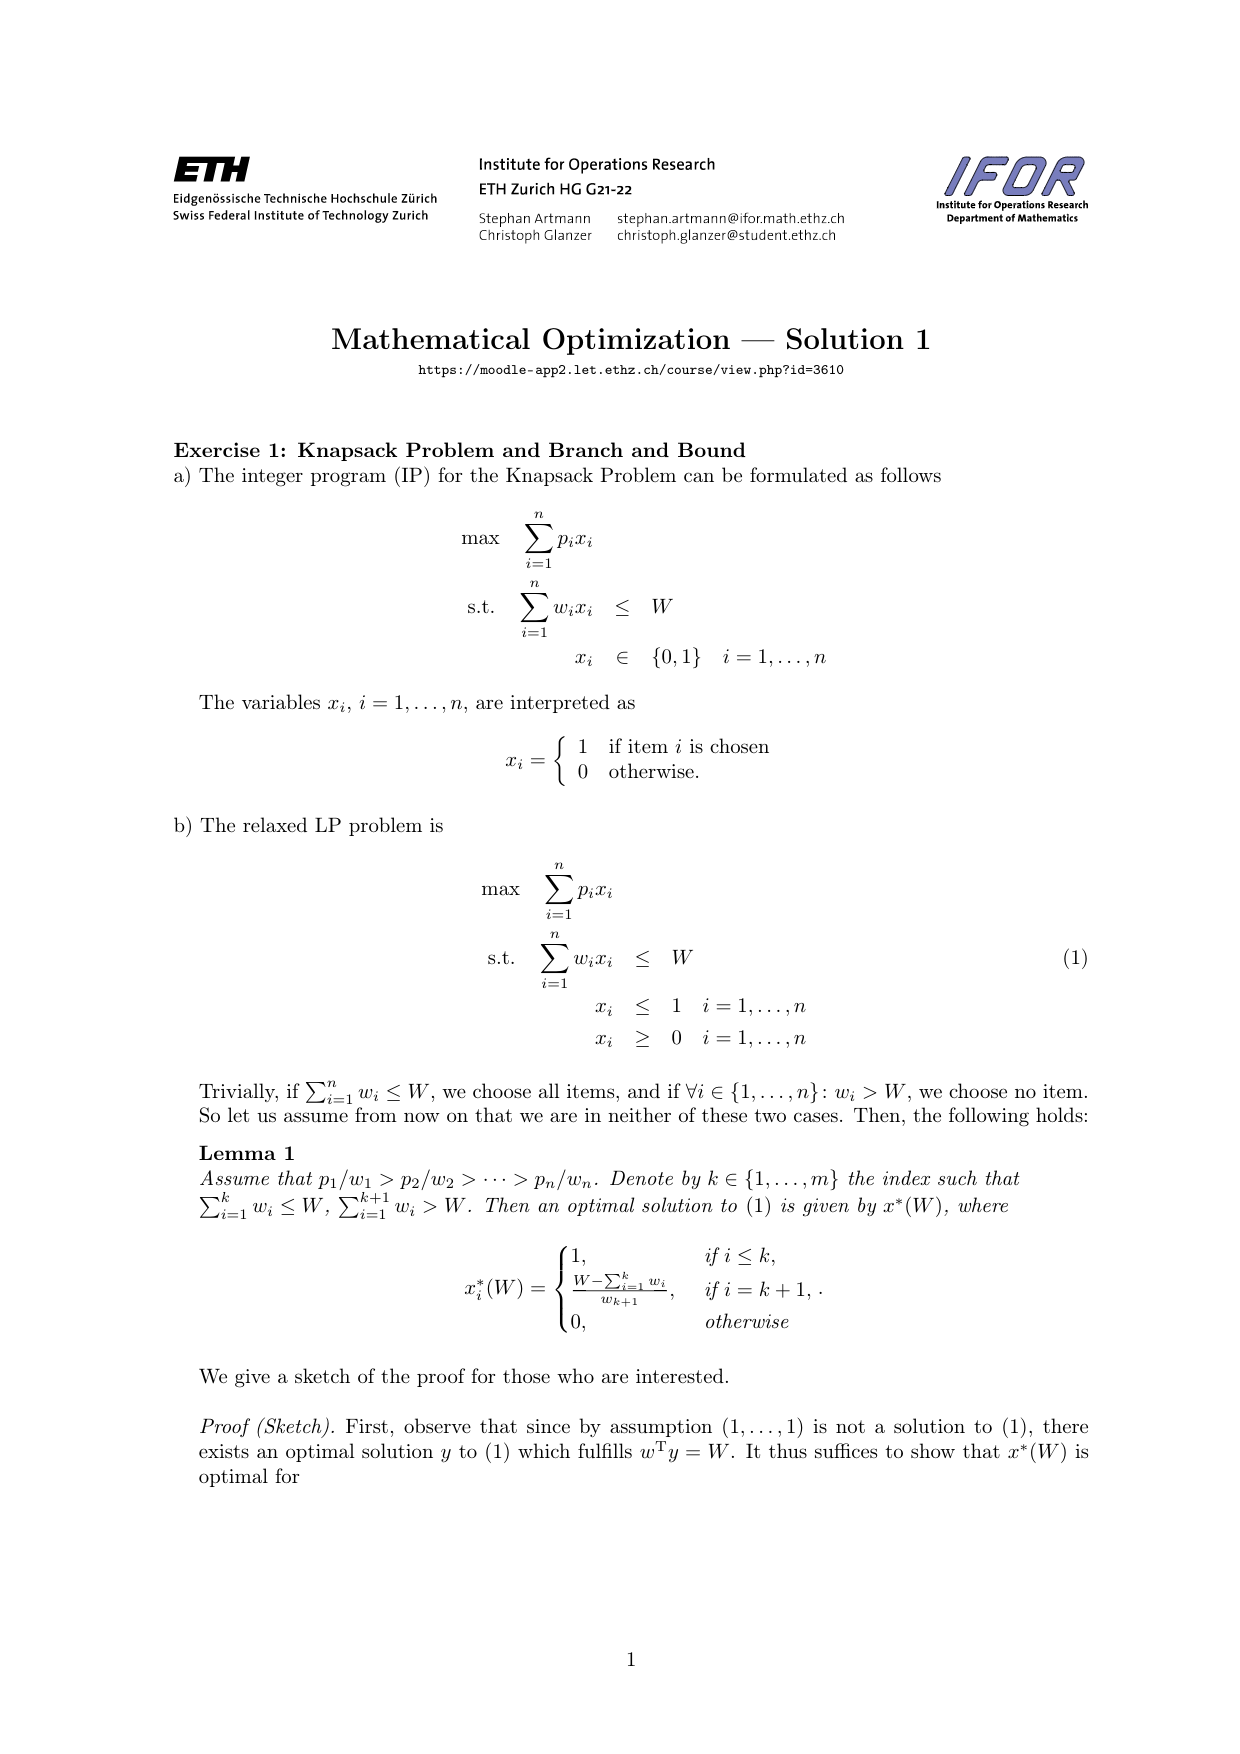
\includepdf[pages={1-4}]{docs/assignments-solutions/solution1.pdf}

\subsection{Assignment 02}
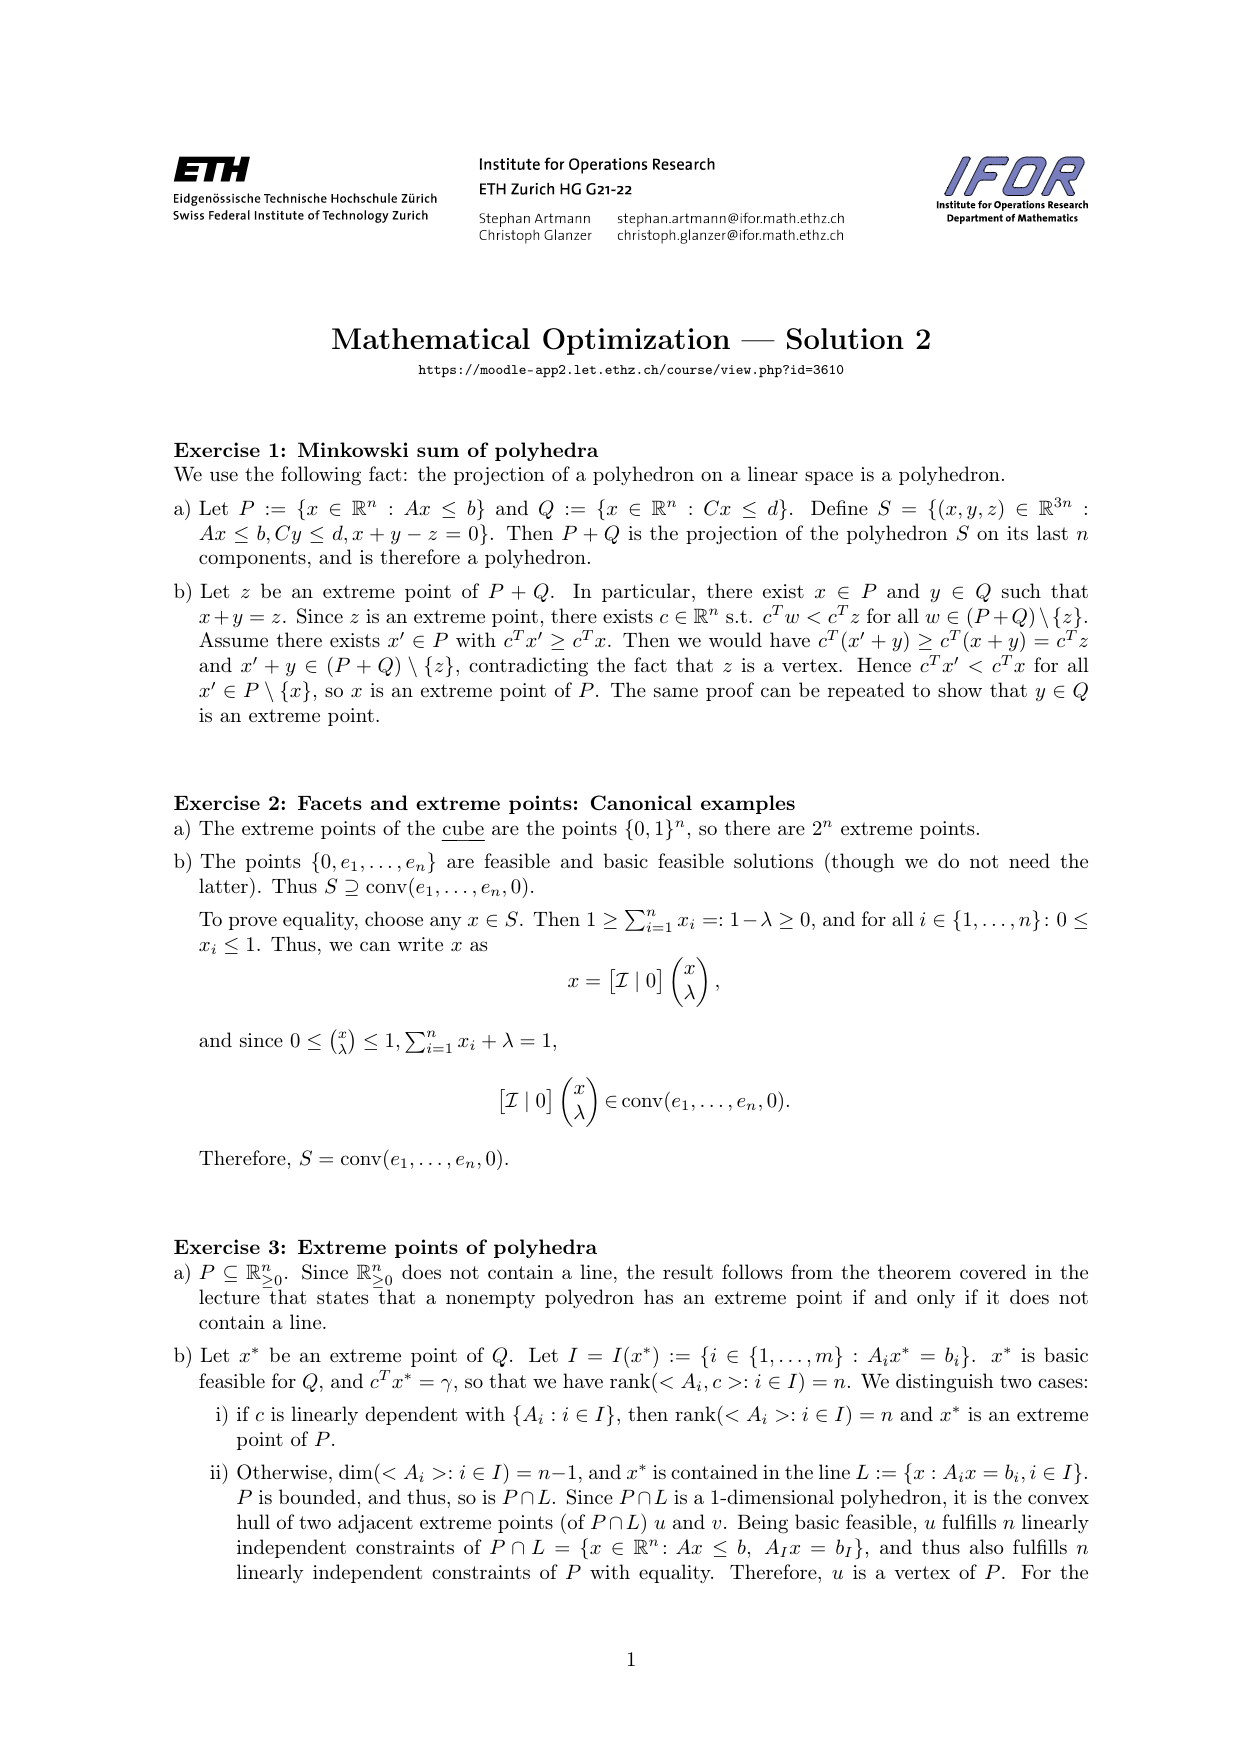
\includepdf[pages={1-2}]{docs/assignments-solutions/solution2.pdf}

\subsection{Assignment 03}
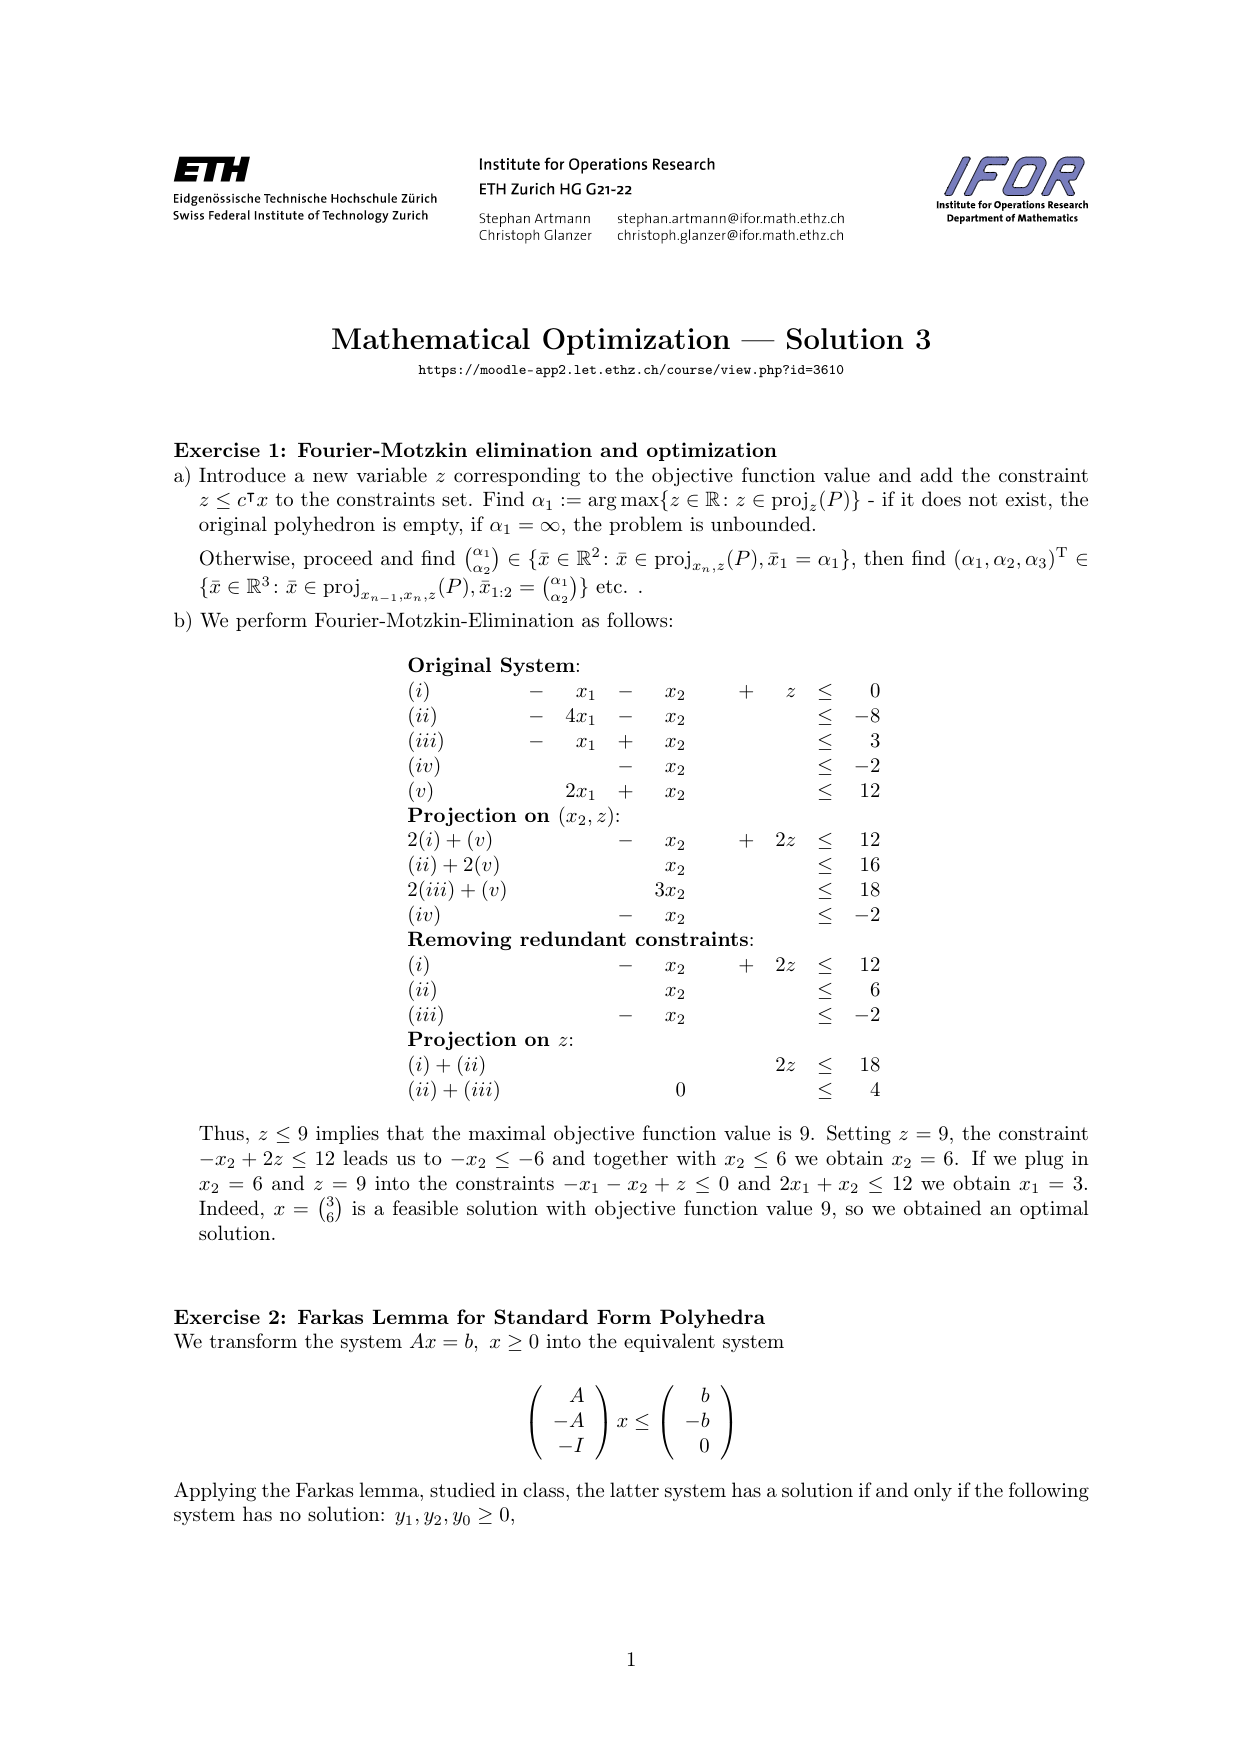
\includepdf[pages={1-3}]{docs/assignments-solutions/solution3.pdf}

\subsection{Assignment 04}
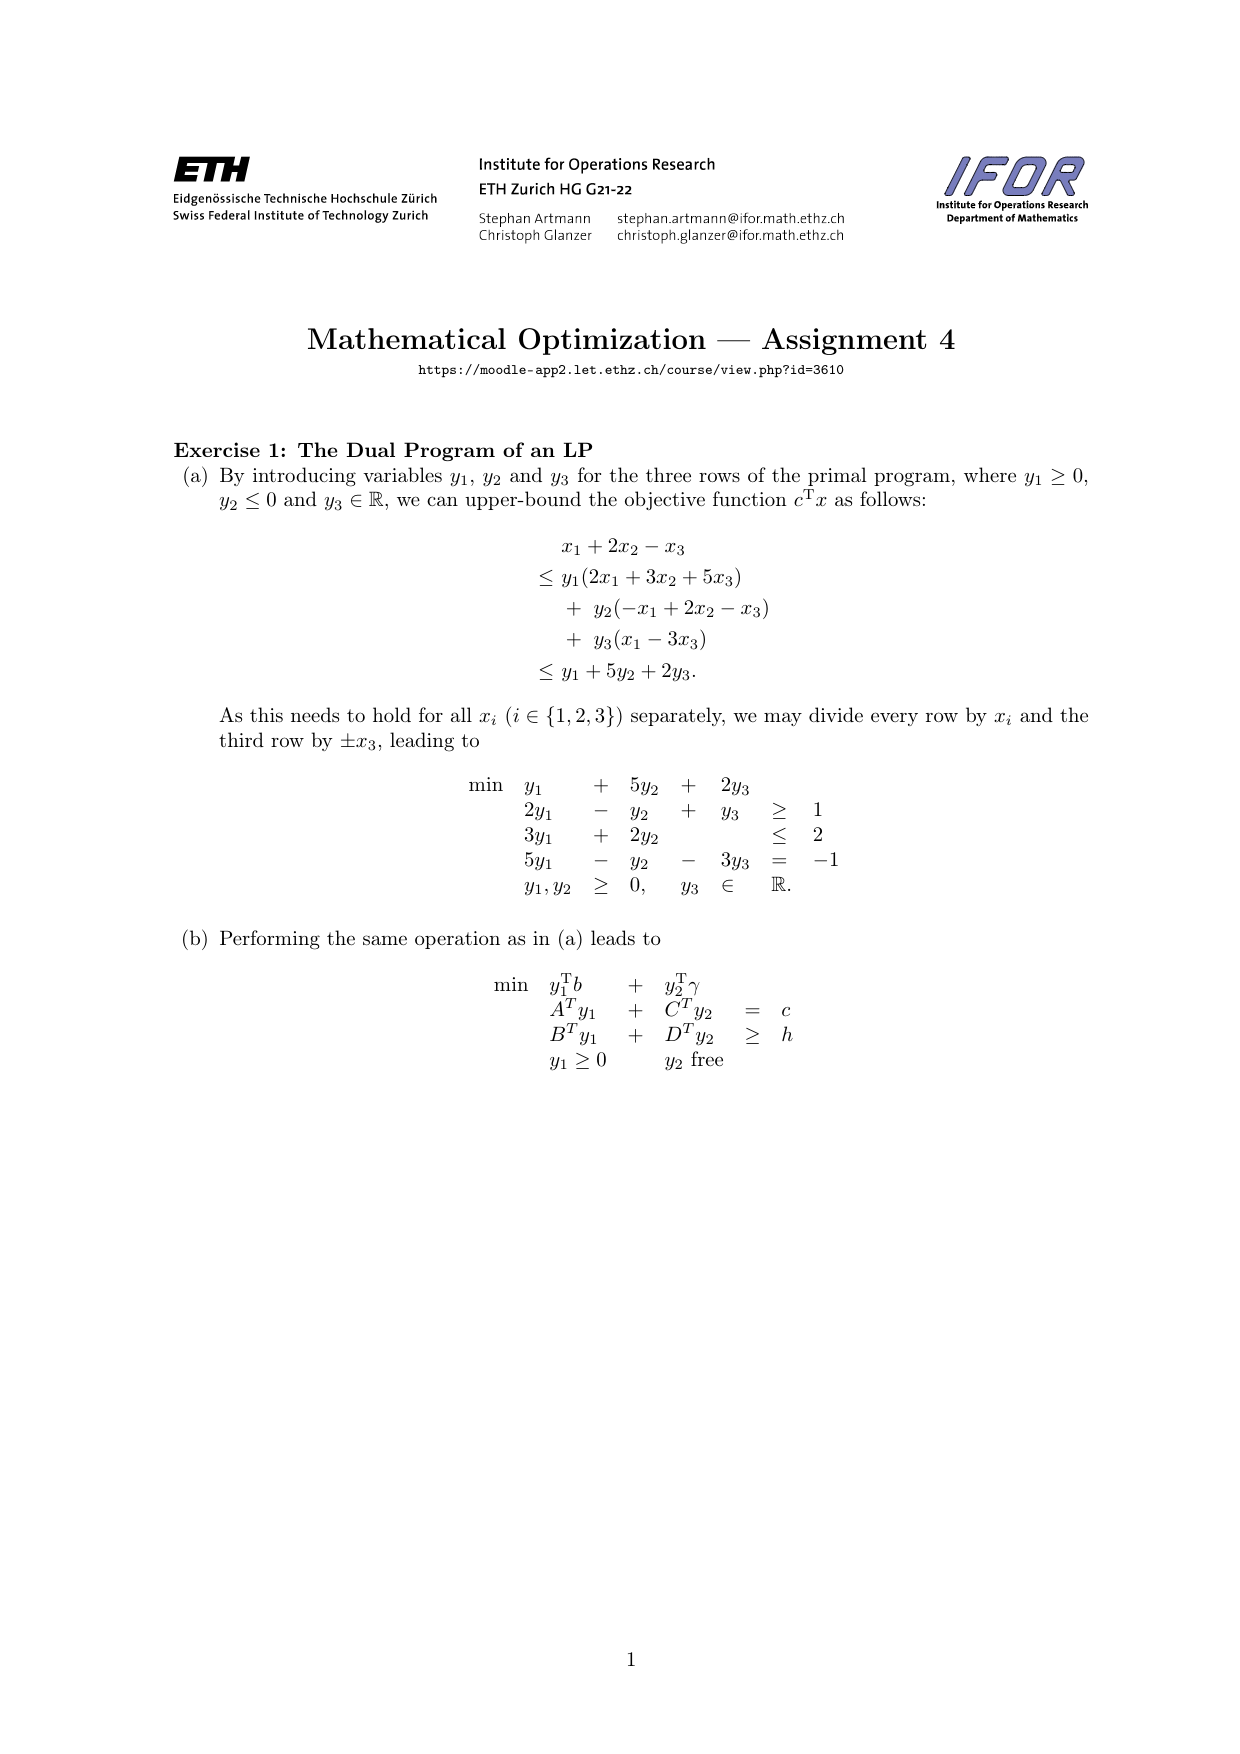
\includepdf[pages={1-4}]{docs/assignments-solutions/solution4.pdf}

\subsection{Assignment 05}
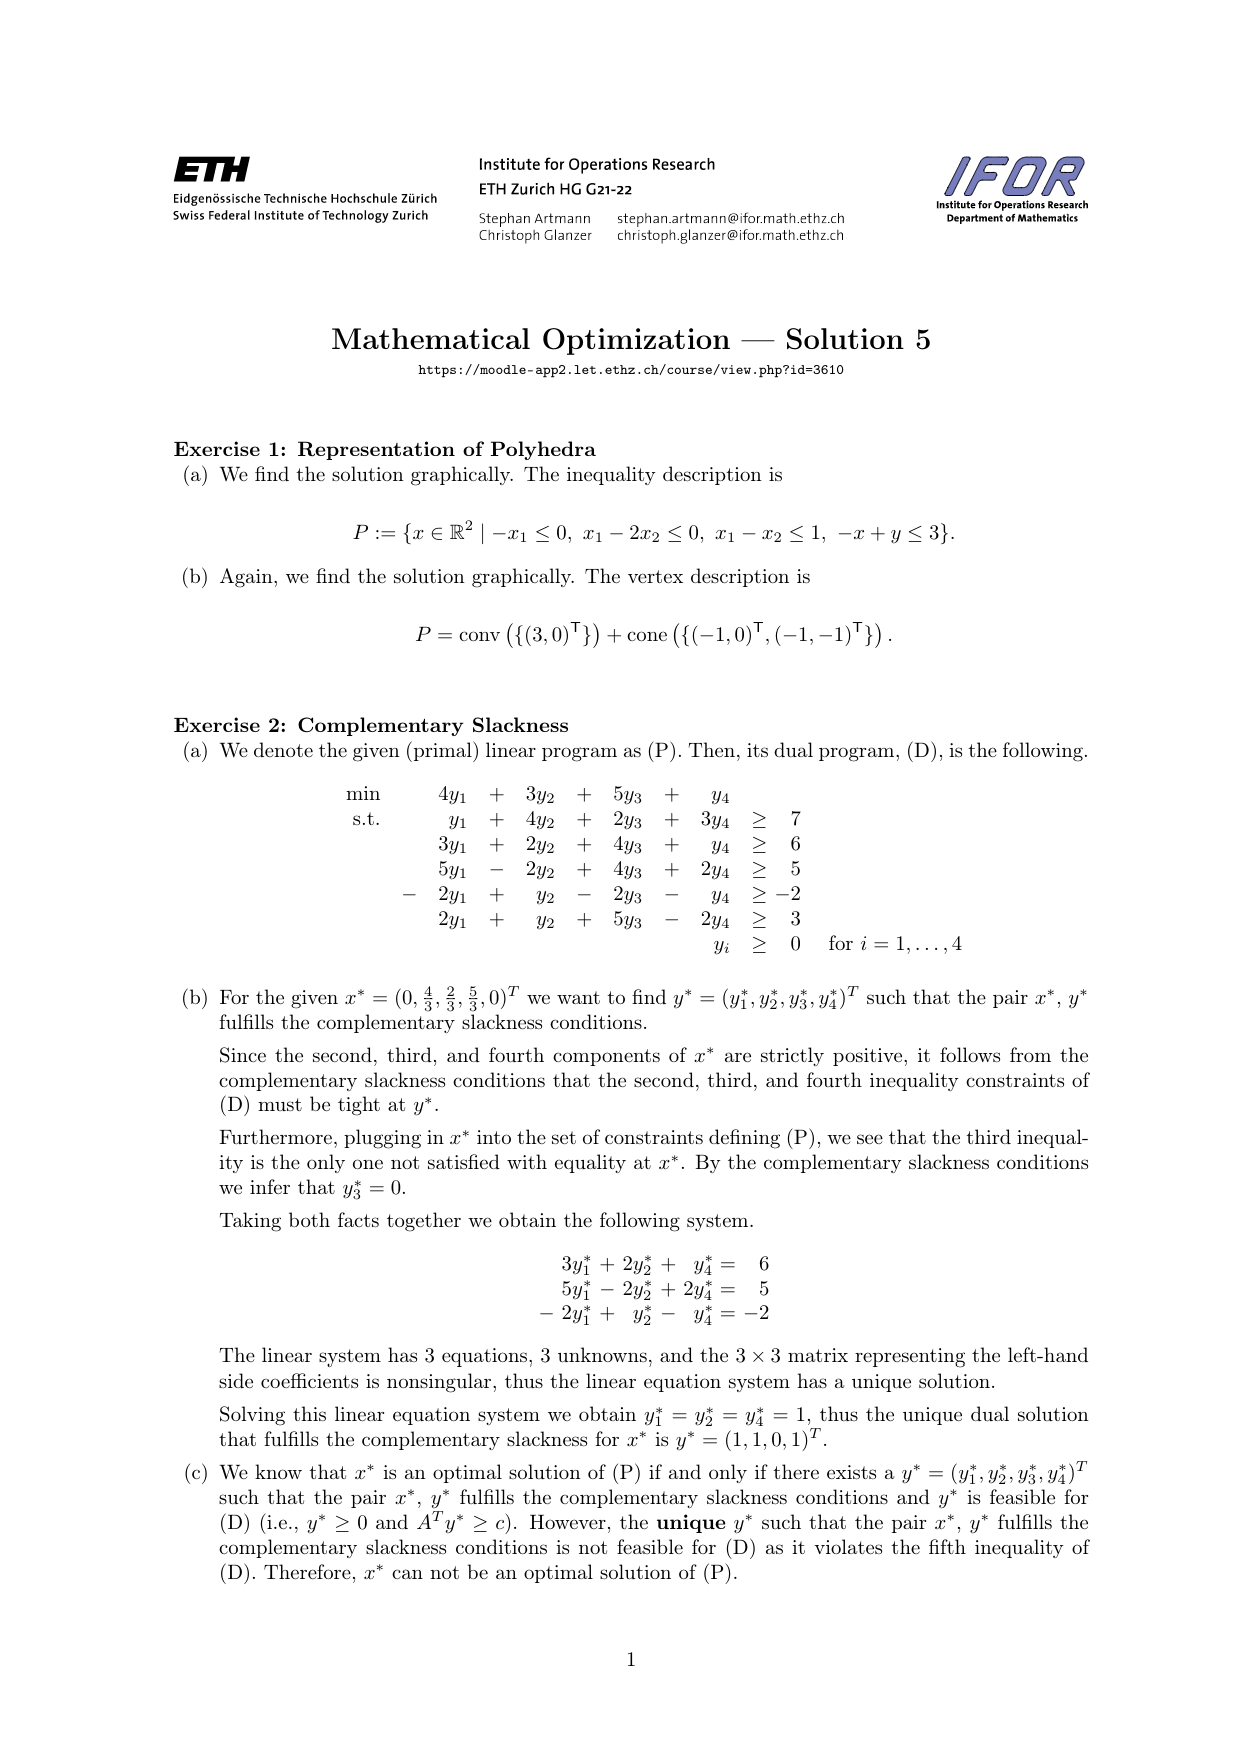
\includepdf[pages={1-4}]{docs/assignments-solutions/solution5.pdf}

\subsection{Assignment 06}
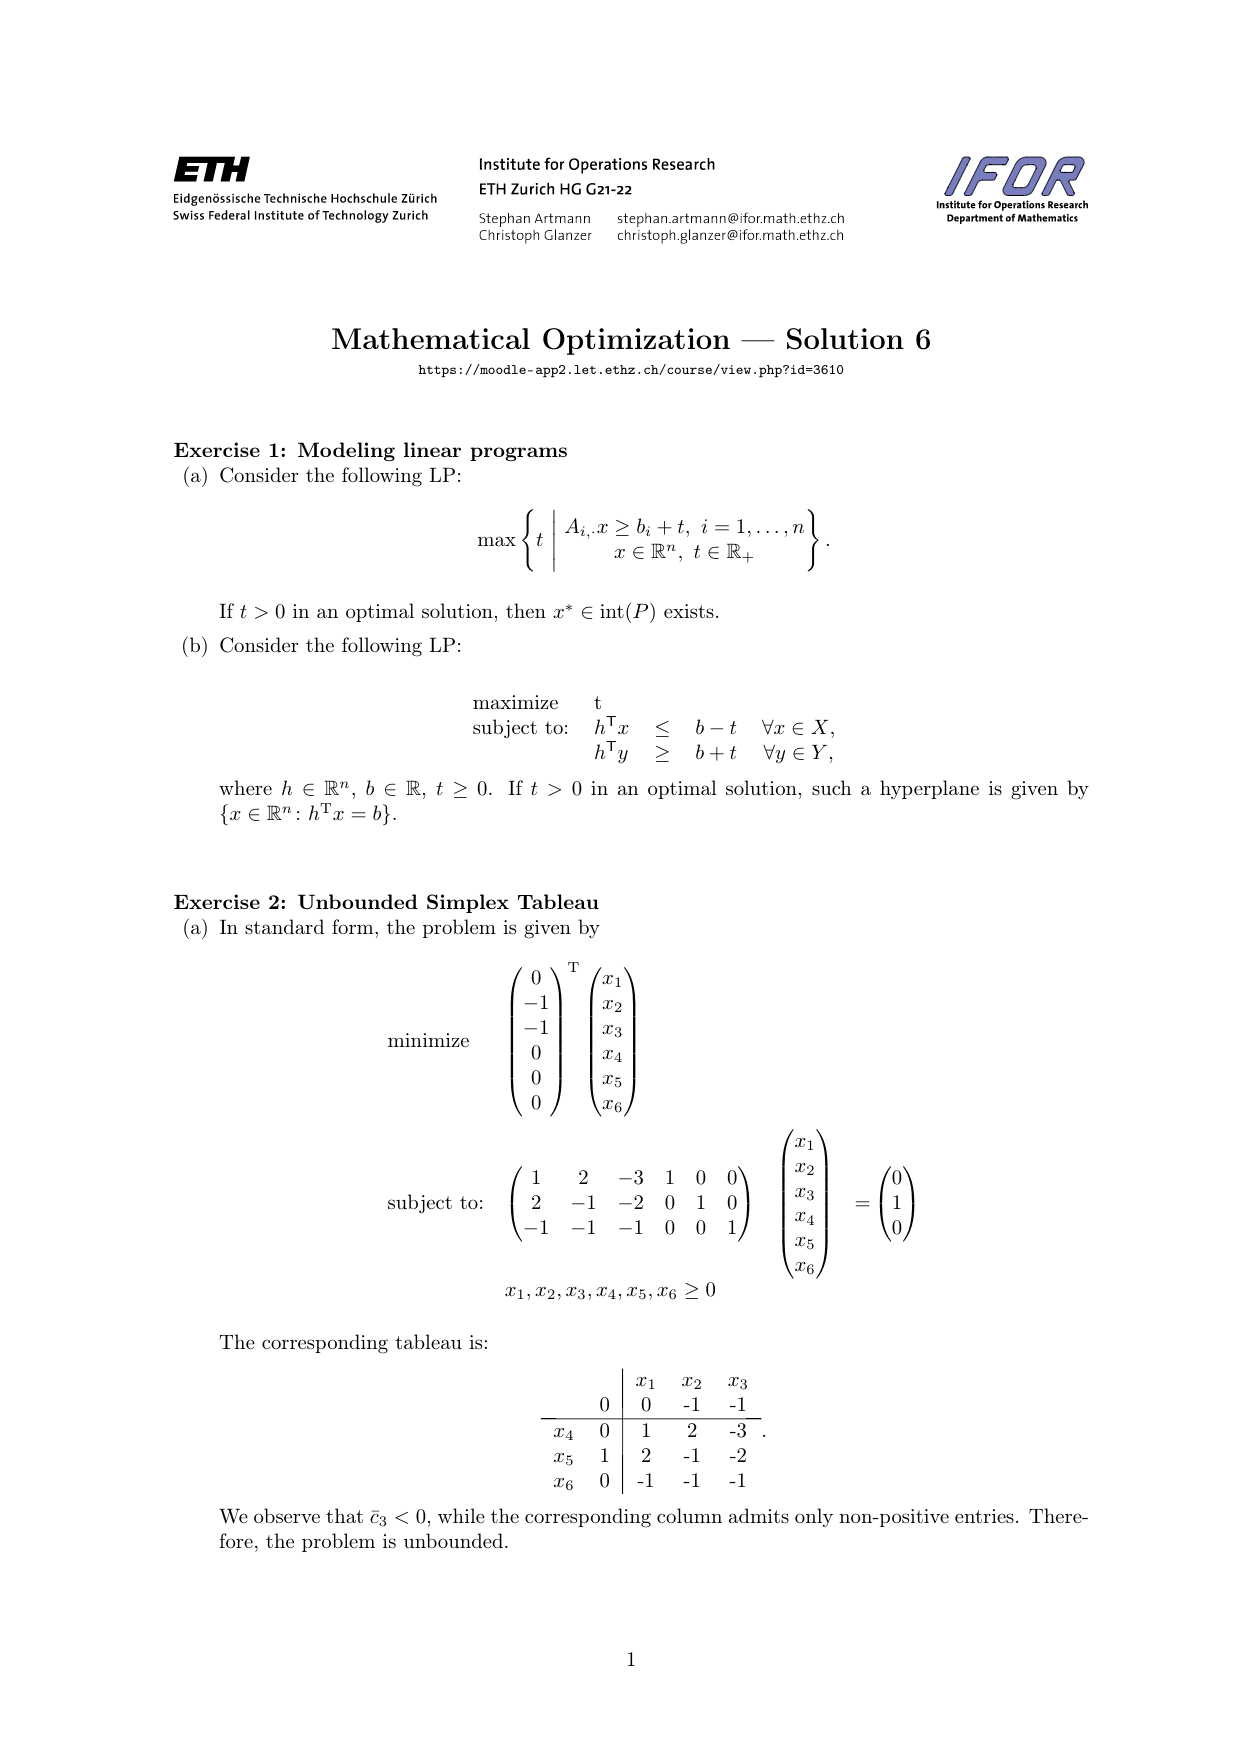
\includepdf[pages={1-3}]{docs/assignments-solutions/solution6.pdf}

\subsection{Assignment 07}
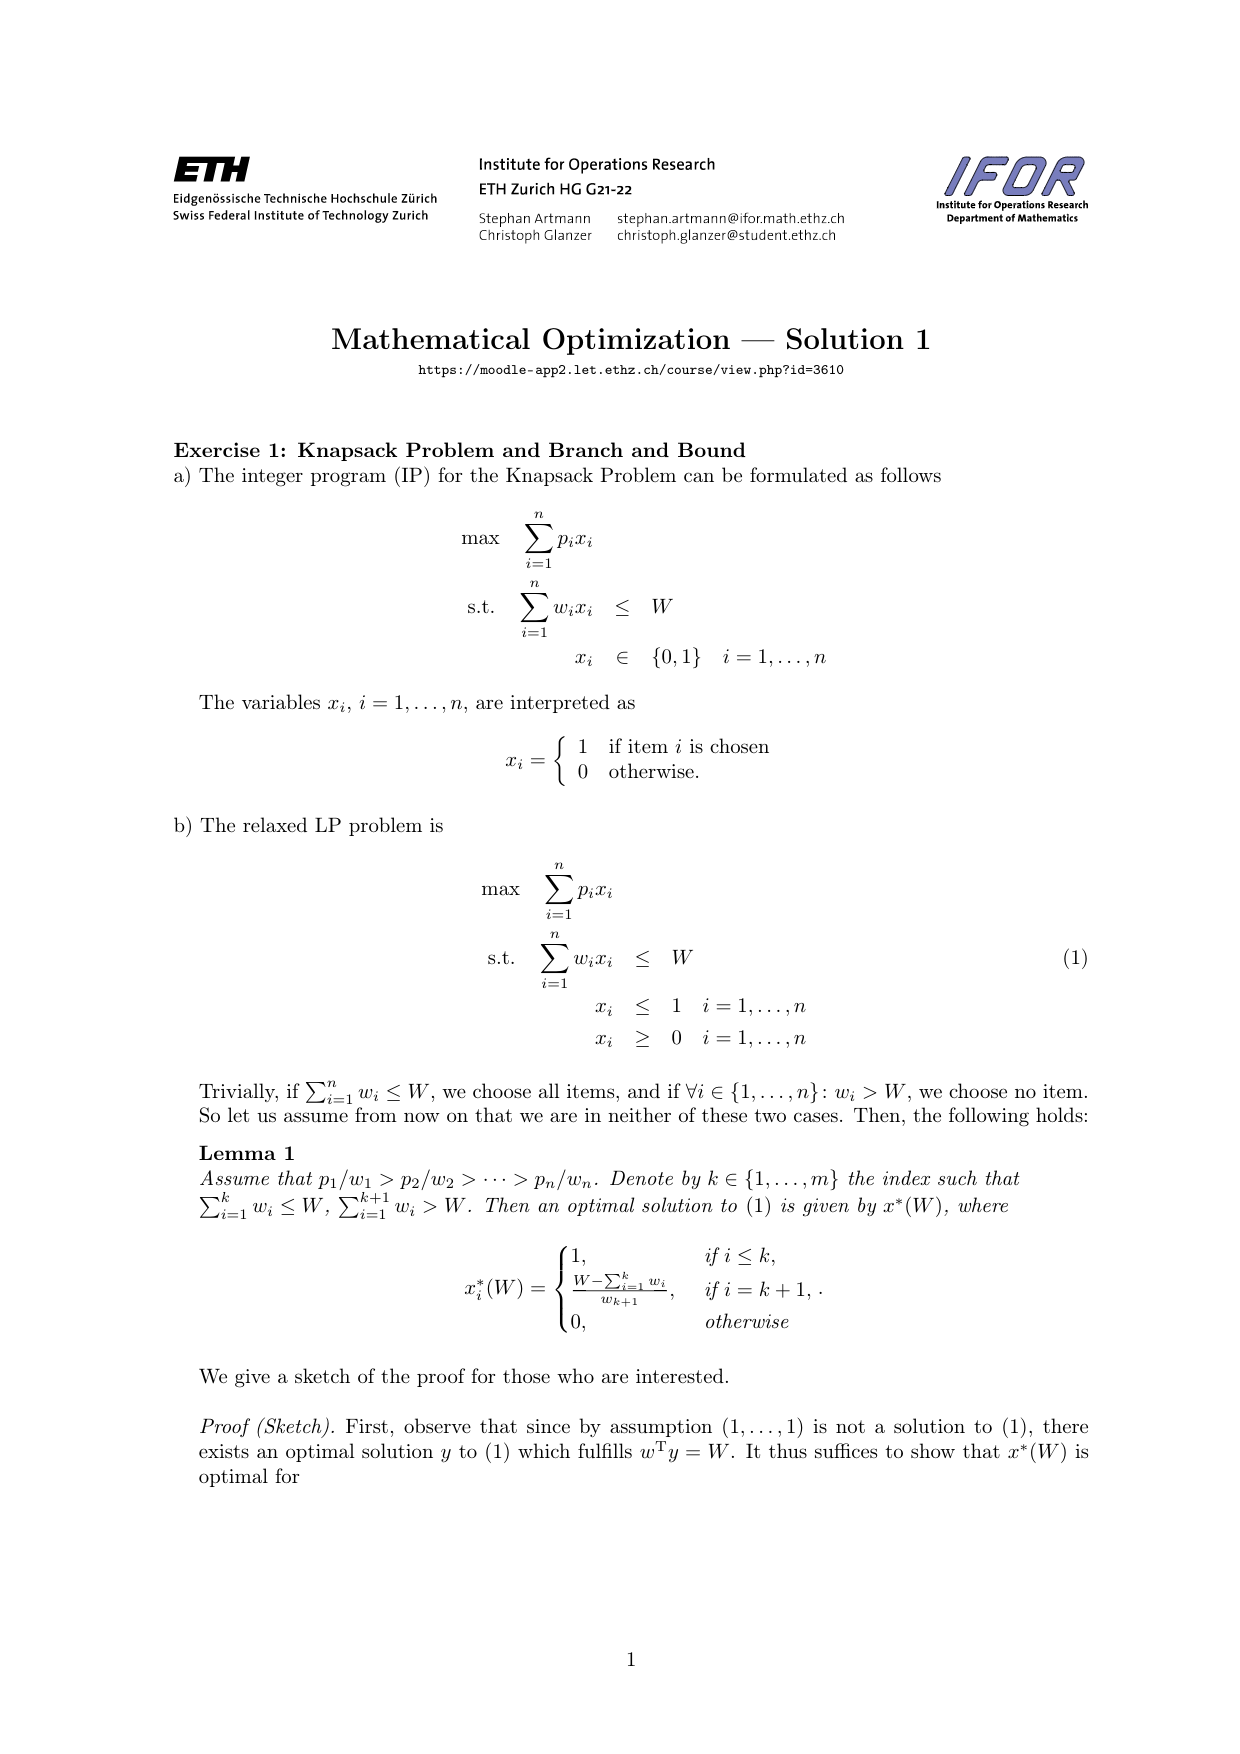
\includepdf[pages={1-3}]{docs/assignments-solutions/solution1.pdf}

\subsection{Assignment 08}
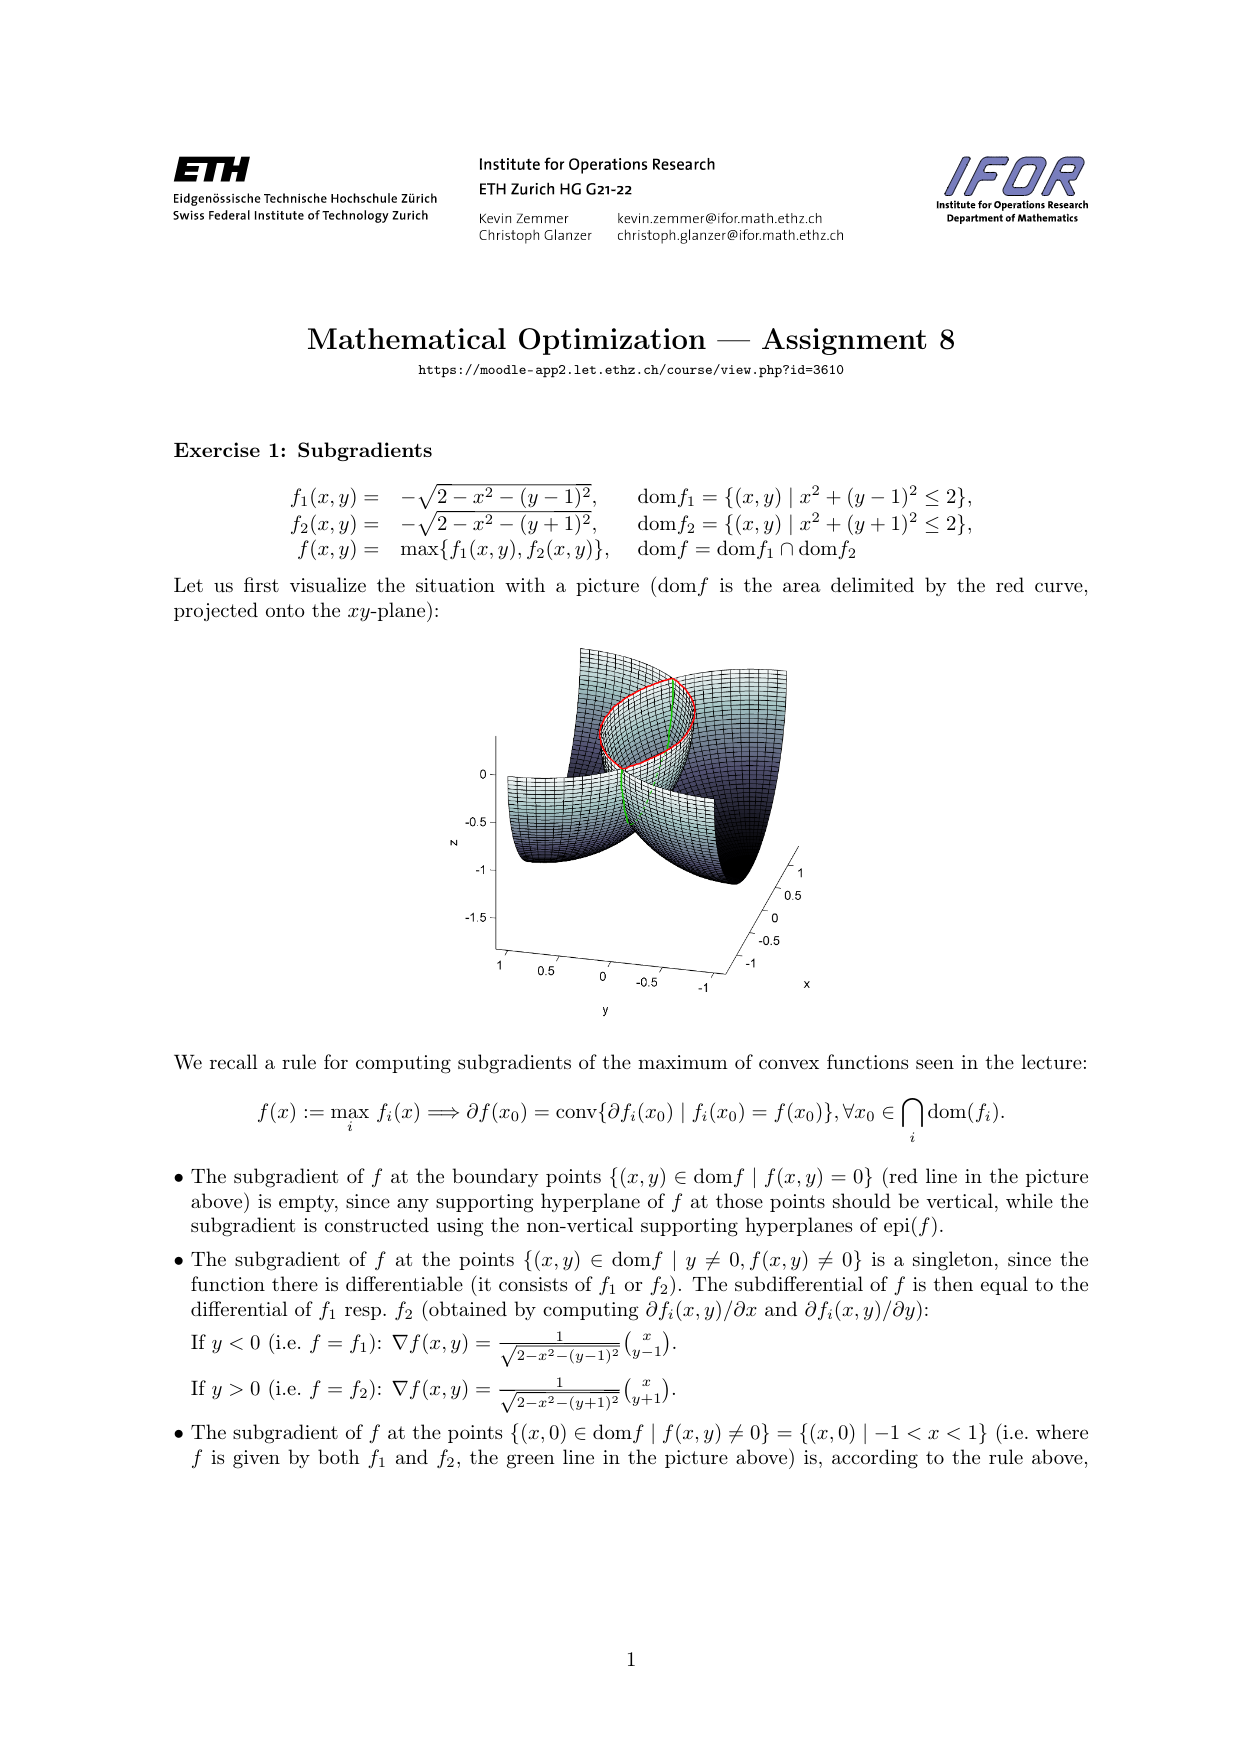
\includepdf[pages={1-2}]{docs/assignments-solutions/solution8.pdf}

\subsection{Assignment 09}
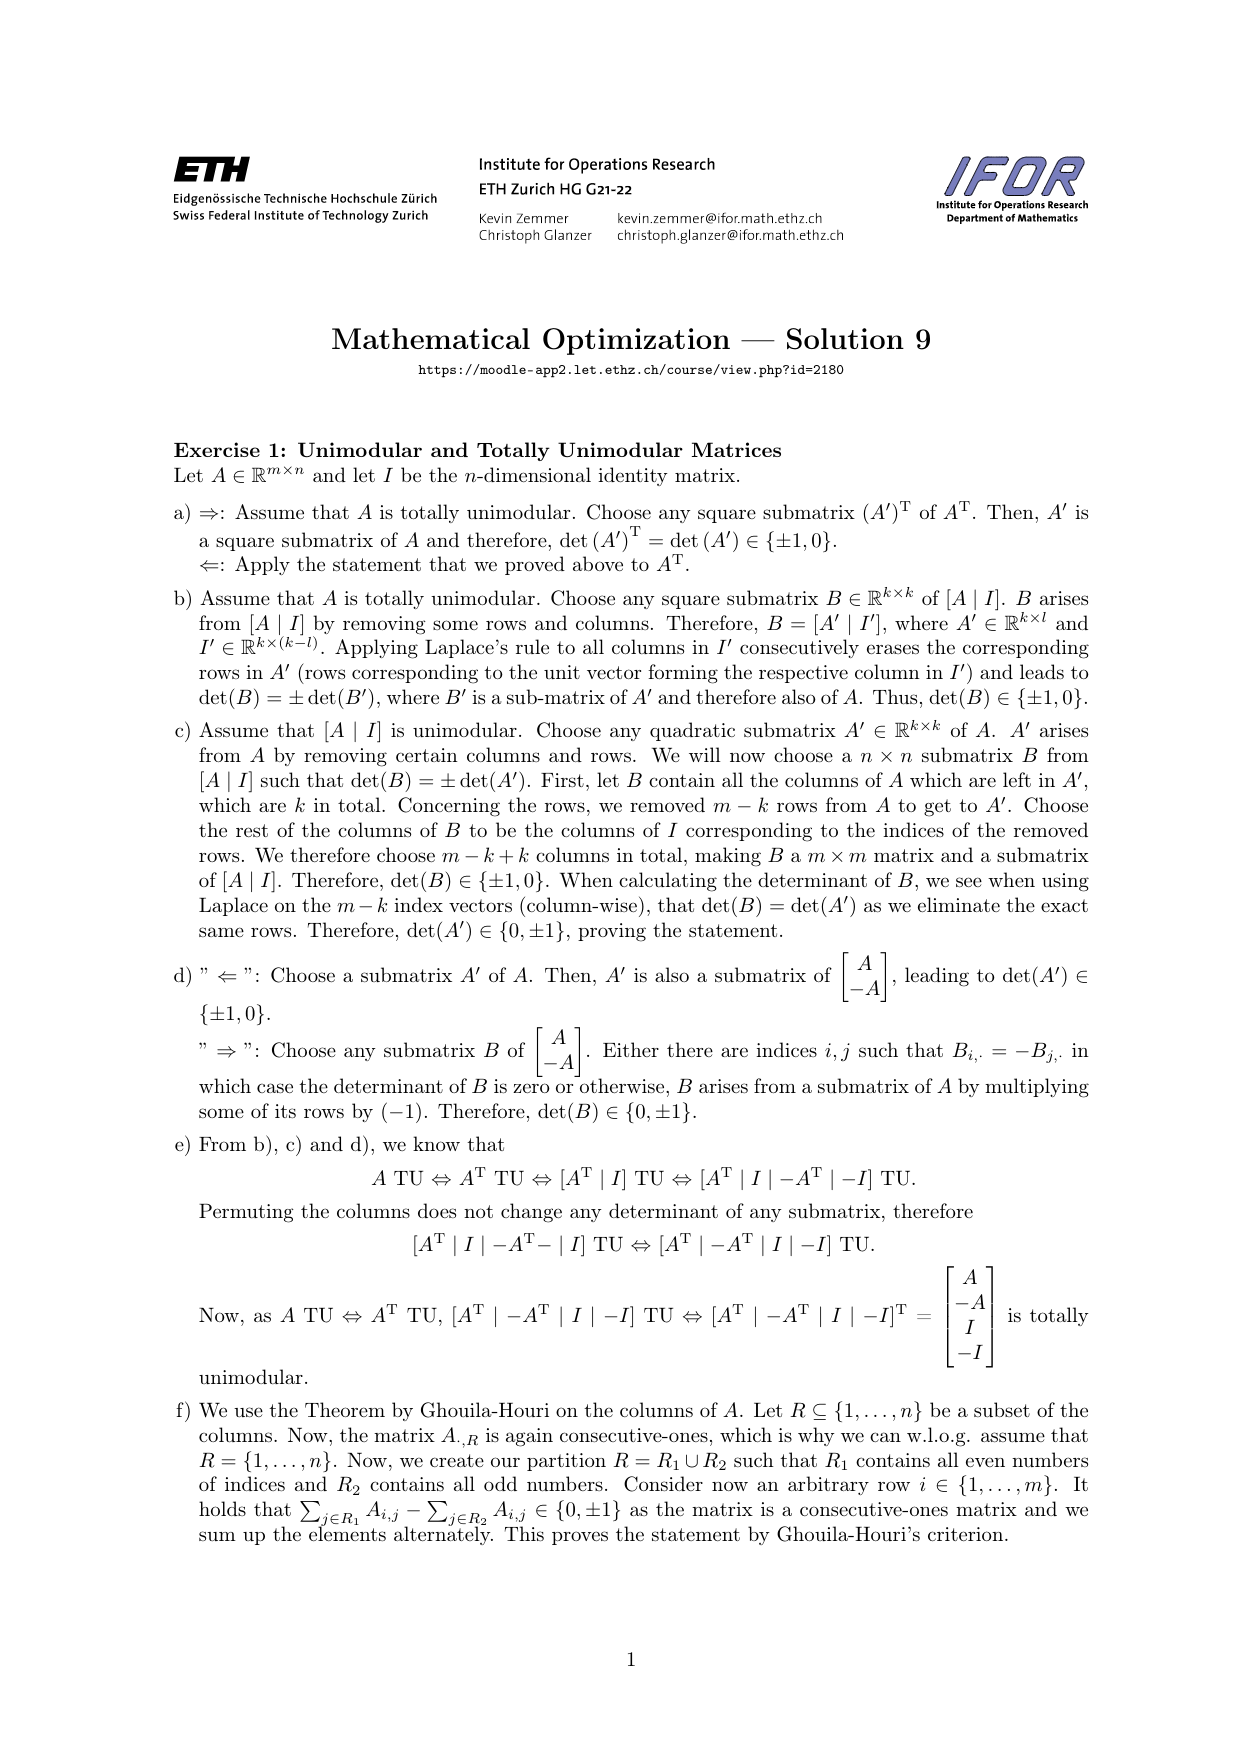
\includepdf[pages={1-2}]{docs/assignments-solutions/solution9.pdf}

\subsection{Assignment 10}
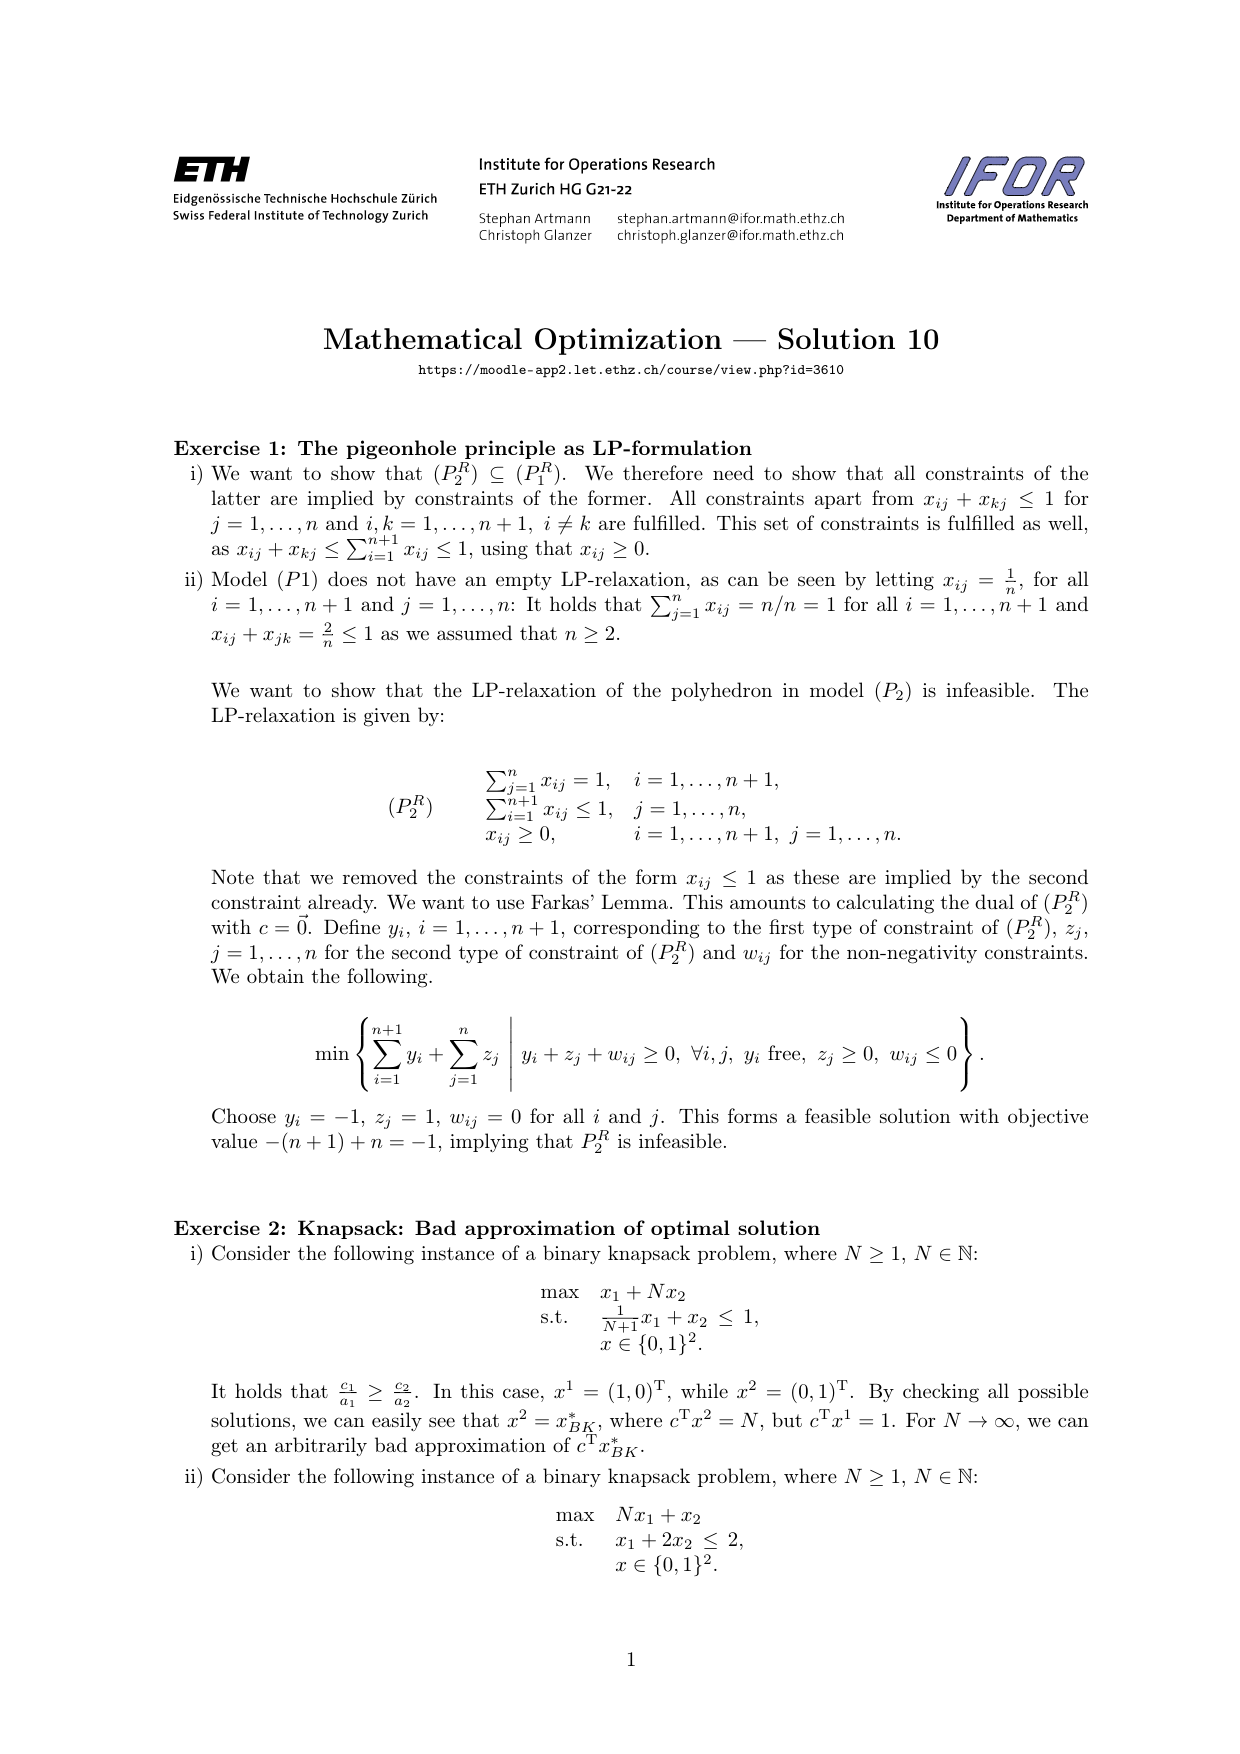
\includepdf[pages={1-2}]{docs/assignments-solutions/solution10.pdf}

\subsection{Assignment 11}
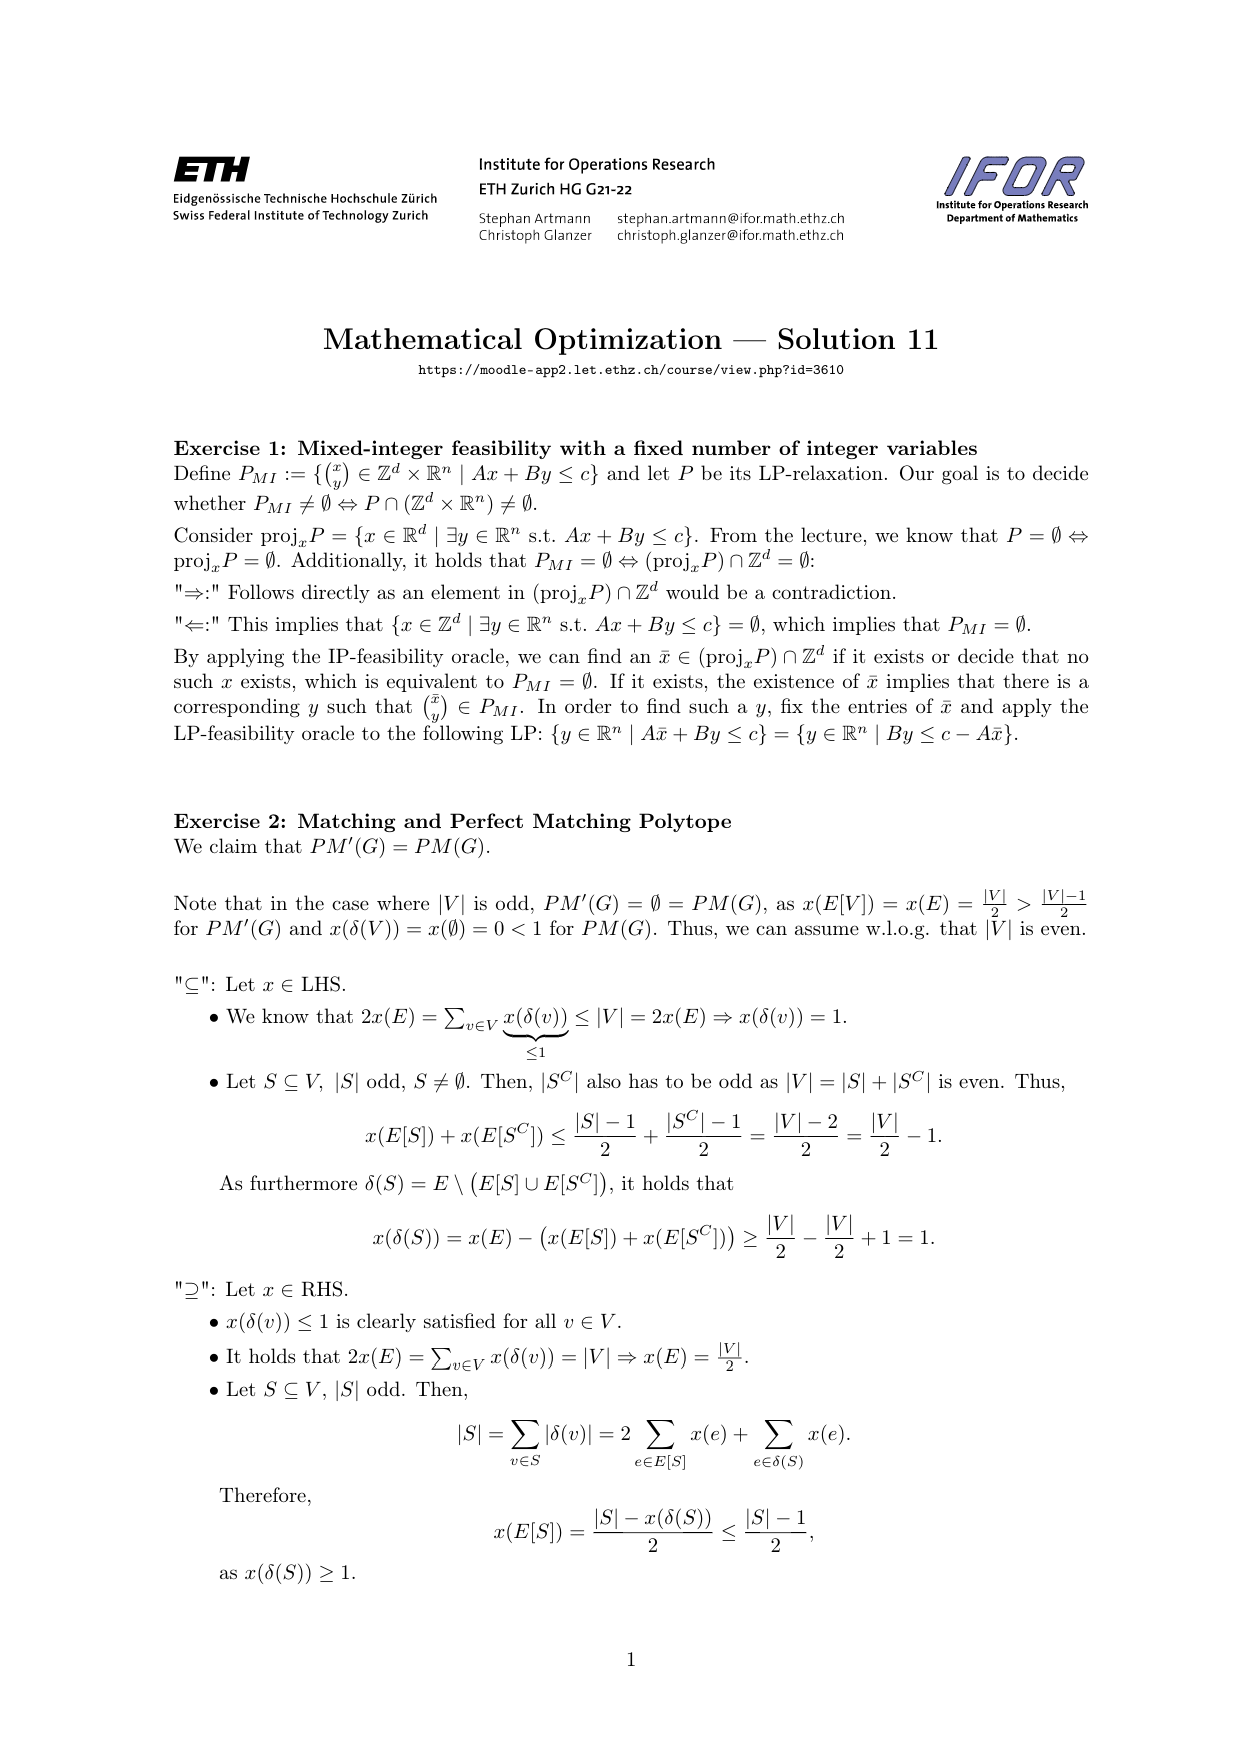
\includepdf[pages={1-2}]{docs/assignments-solutions/solution11.pdf}

\subsection{Assignment 12}
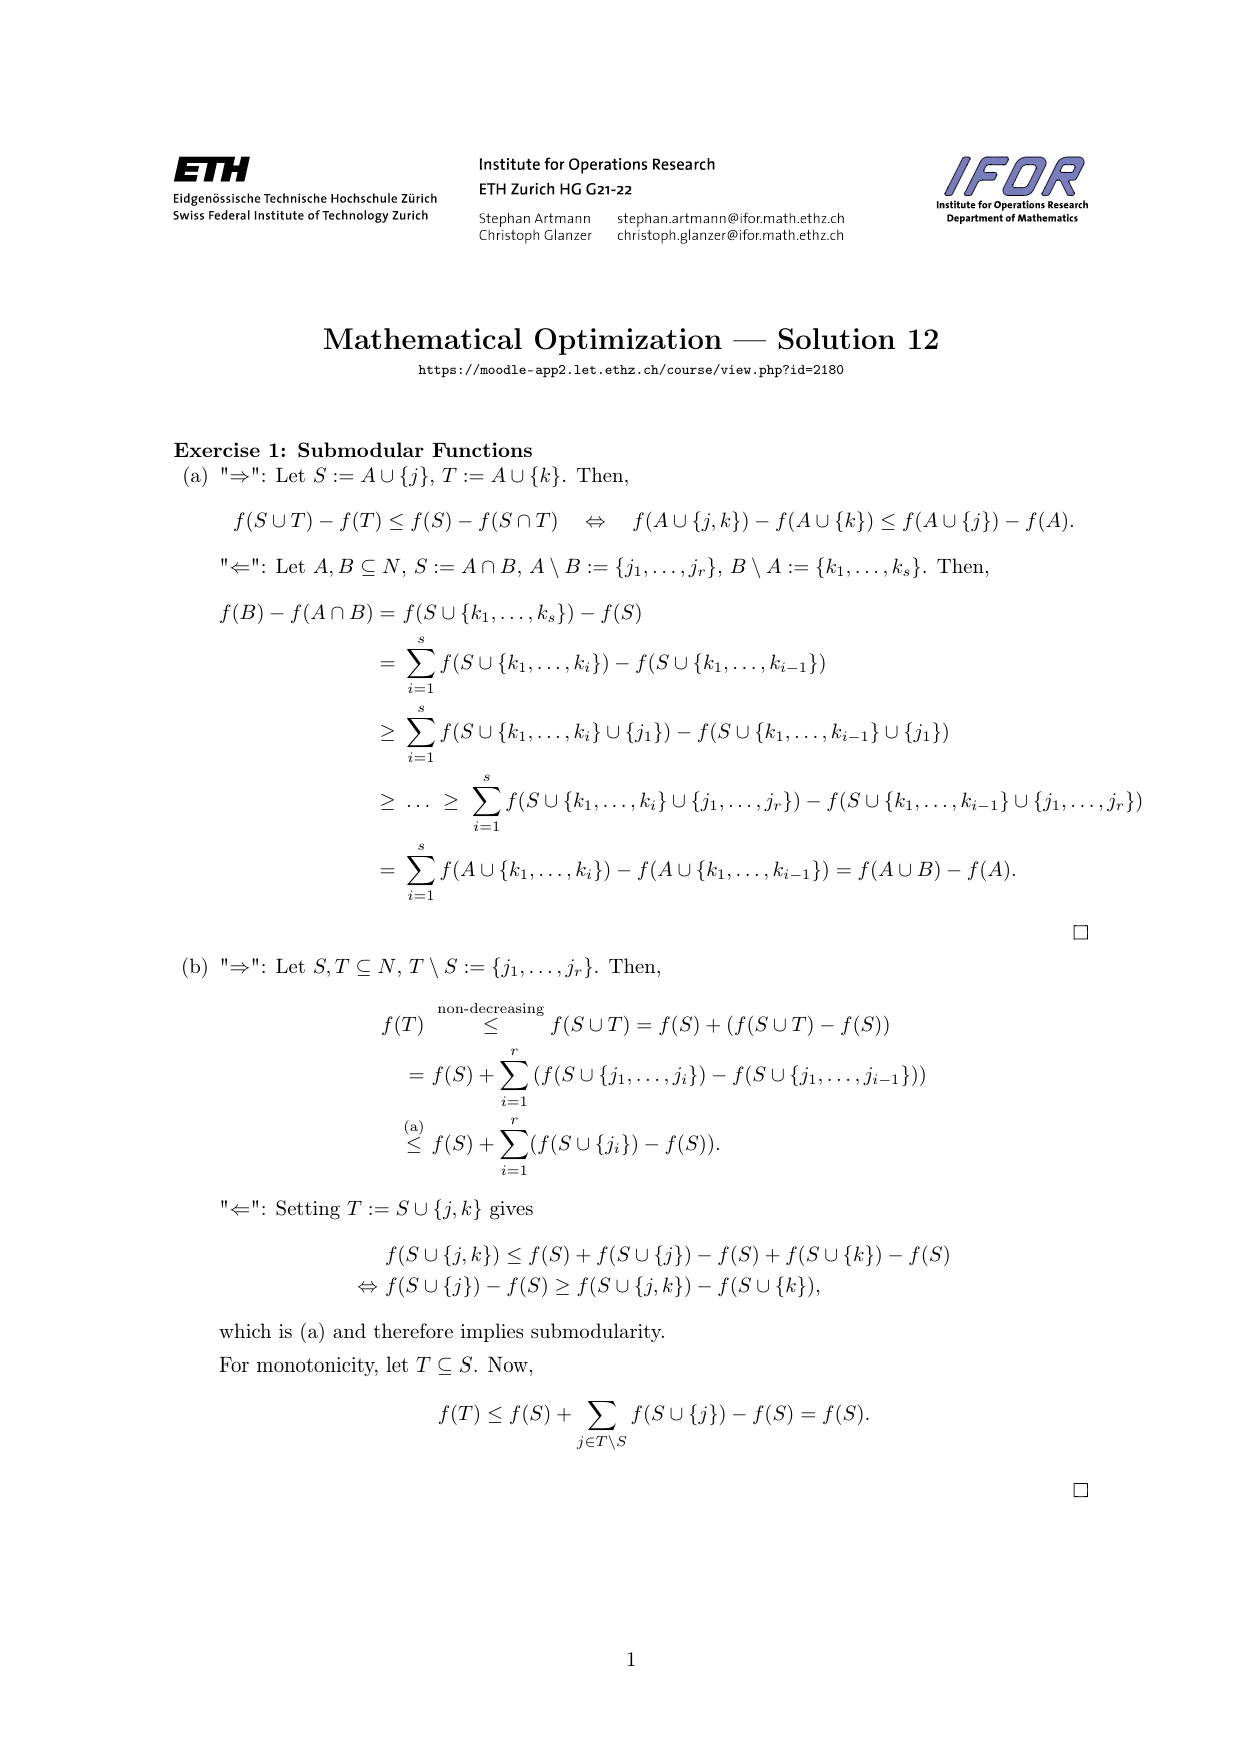
\includepdf[pages={1-2}]{docs/assignments-solutions/solution12.pdf}

\pagebreak

%\pagebreak
%\def\cheatsheet{2014}
%\subfile{15-Cheatsheet2014-BE.tex}

\subfile{27-Glossary.tex}

\subfile{28-TODO.tex}

\end{document}
